%\documentclass[10pt]{beamer}
\documentclass[10pt,aspectratio=169,usenames,dvipsnames]{beamer}

\usetheme[progressbar=frametitle]{metropolis}
\usepackage{appendixnumberbeamer}

\usepackage{booktabs}
\usepackage[scale=2]{ccicons}

\usepackage{pgfplots}
\usepgfplotslibrary{dateplot}

\usepackage{xspace}
\newcommand{\themename}{\textbf{\textsc{metropolis}}\xspace}

\usepackage{graphicx}

\setbeamertemplate{enumerate items}[circle]

\usepackage{pict2e}

\usepackage{media9}

\usepackage{amsmath}

\usepackage{mathtools}
\DeclarePairedDelimiter\abs{\lvert}{\rvert}%
\DeclarePairedDelimiter\norm{\lVert}{\rVert}%
\makeatletter
\let\oldabs\abs
\def\abs{\@ifstar{\oldabs}{\oldabs*}}

\usepackage[makeroom]{cancel}

\usepackage{xcolor}
\usepackage{soul}
\newcommand{\mathcolorbox}[2]{\colorbox{#1}{$\displaystyle #2$}}

\title{\textcolor{black}{Mixing induced co}\textcolor{orange}{oling in the solar atmosphere}}
%ABSTRACT: 
\date{}
\author{\textbf{\textcolor{black}{Ben Snow}}}
\institute{\textcolor{black}{University of Exeter} \\ \textcolor{black}{UKMHD2023, Leeds, 19th May 2023.}}


\titlegraphic{\vspace{-0.7cm} \hspace{-1.3cm}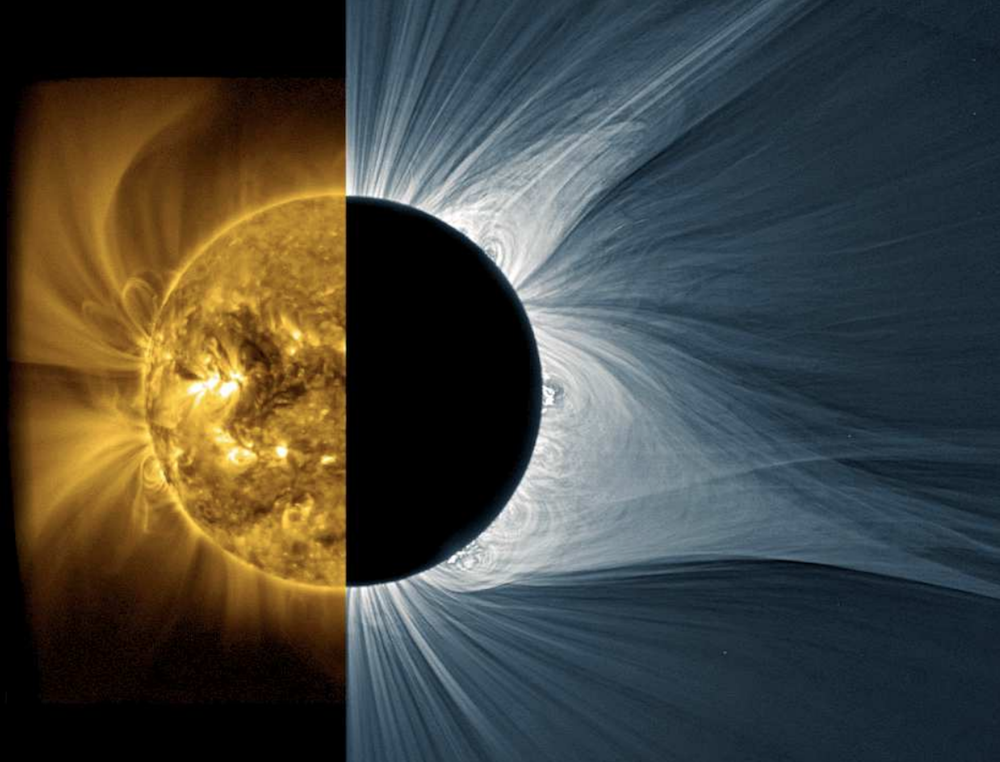
\includegraphics[width=\paperwidth,height=\paperheight]{2023Dundee/Figures/SolarCoronaDouble.png}}

\begin{document}

\maketitle

\begin{frame}{Solar atmosphere}
\begin{columns}
\begin{column}{0.5\textwidth}
\begin{itemize}
    \item The Sun gets hotter as you move up in the solar atmosphere - why?
    \item Magnetic energy dominates thermal energy.
    \item Dissipating a little bit of magnetic energy can result in significant heating
    \item Most of the energy is in the potential field component, so how does free magnetic energy get into the corona?
    %\item But it is not this simple, most magnetic energy is in the potential field component, so how do we get free magnetic energy into the corona?
\end{itemize}
\end{column}
\begin{column}{0.5\textwidth}
%\includegraphics[width=0.32\linewidth]{Figures/Crab_Nebula.jpeg}
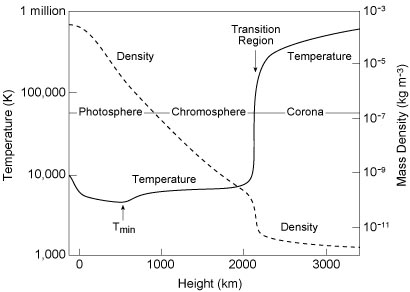
\includegraphics[width=0.95\linewidth]{2023Dundee/Figures/valc.png} \\
%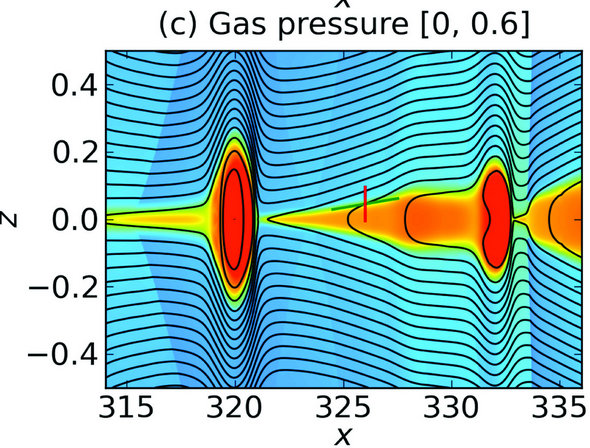
\includegraphics[width=0.95\linewidth]{2023RAS/Figures/shibyama.png}
%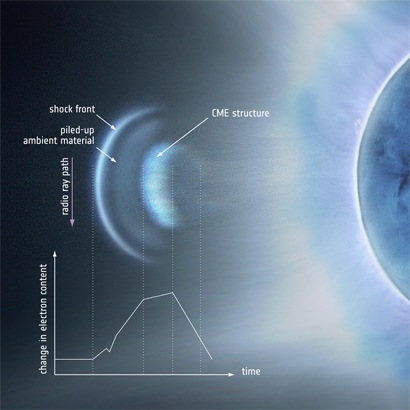
\includegraphics[width=0.32\linewidth]{Figures/cmesketch.jpg}
\end{column}
\end{columns}
\end{frame}

% \begin{frame}{Energising the corona}
% \centering
% 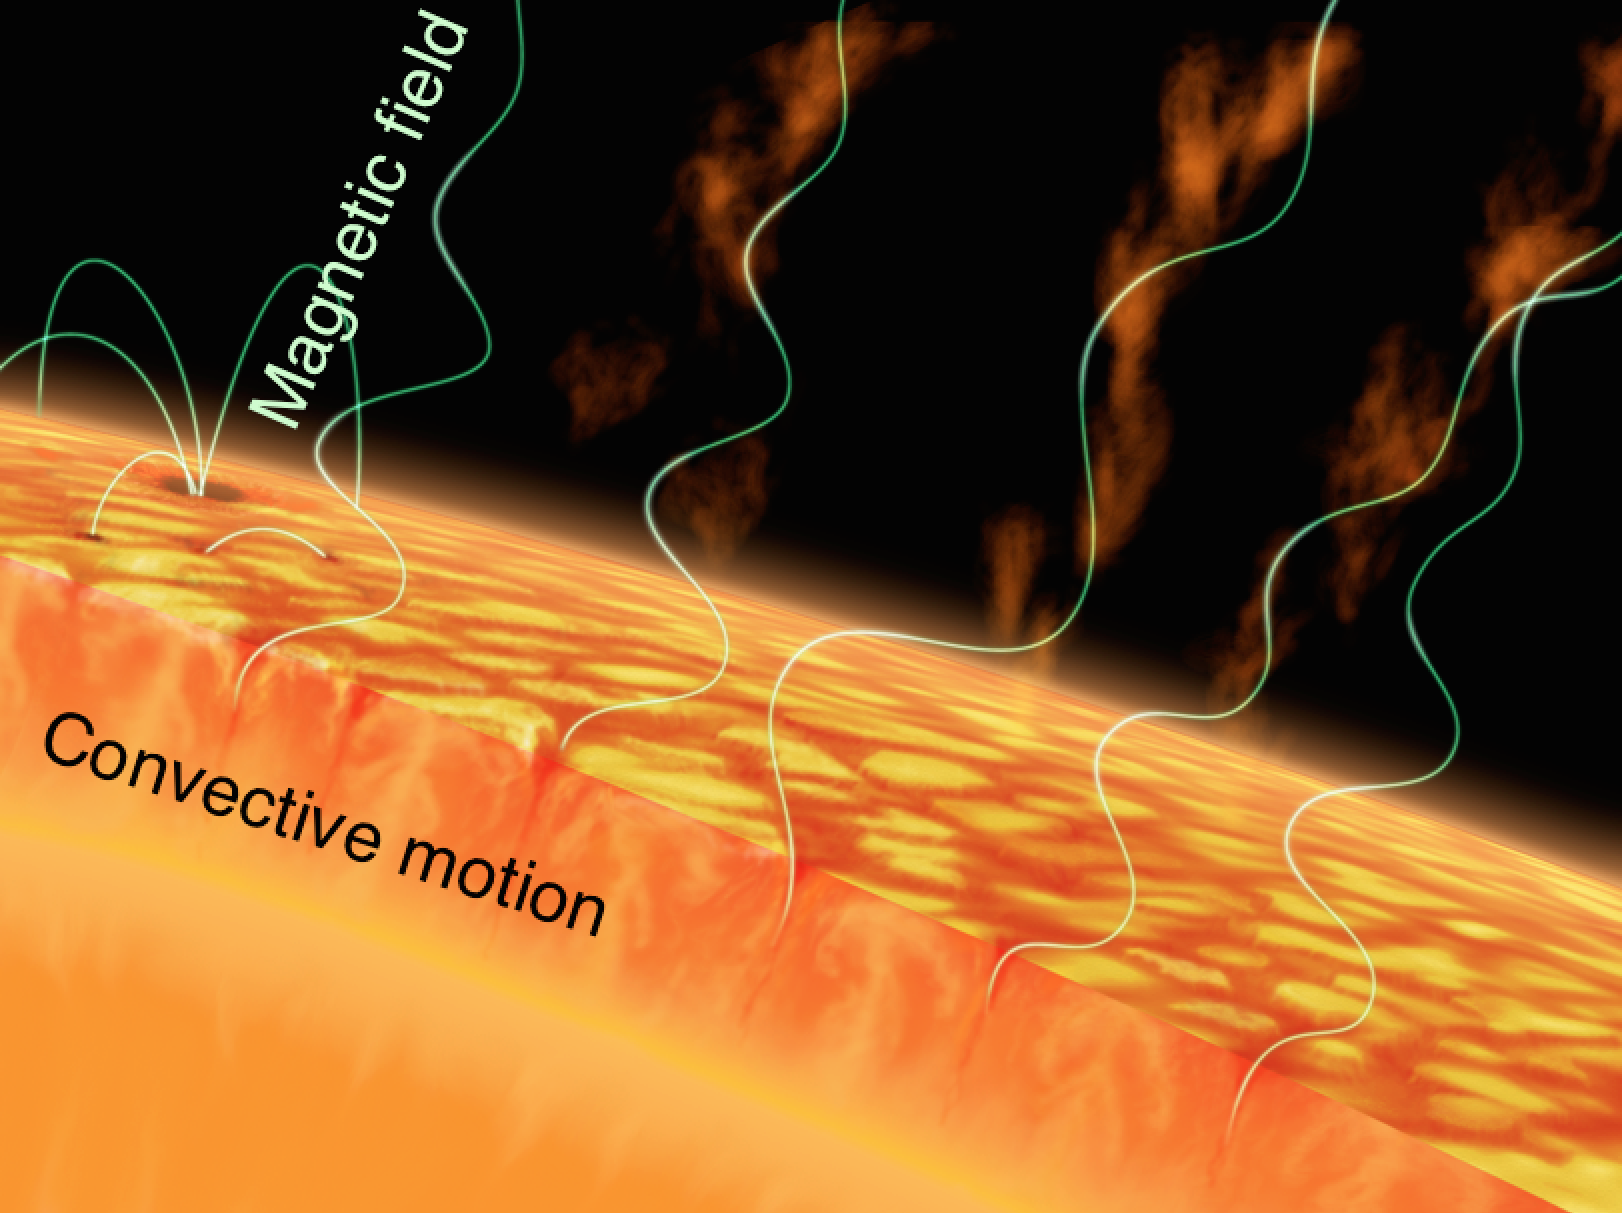
\includegraphics[width=0.45\linewidth]{2023Dundee/Figures/waveheating.png} 
% 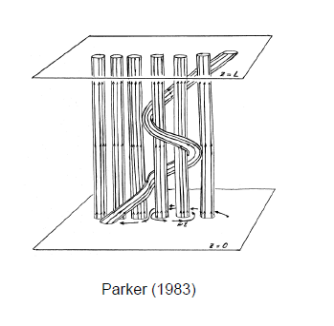
\includegraphics[width=0.45\linewidth,clip=true,trim=0.0cm 1.0cm 0.0cm 0.0cm]{2023Dundee/Figures/reconnection.png}
% %\begin{columns}
% %\begin{column}{0.4\textwidth}
% \begin{itemize}
%     % \item Solar chromosphere is partially ionised.
%     % \item Understanding two-fluid shocks is fundamental to understanding energy transfer and heating in the solar chromosphere and corona.
%     %\item AC vs DC
%     \item Main methods for converting magnetic energy into thermal energy are broadly categorised as AC (waves) and DC (reconnection)
%     \item Observations used to infer the heating.
% %    \item Substructure possible.
% \end{itemize}
% %\includegraphics[width=1.0\textwidth,clip=true,trim=1.0cm 1.0cm 1.0cm 1.0cm]{obs_shockloc_contour.png}
% %\end{column}
% %\begin{column}{0.6\textwidth}
% %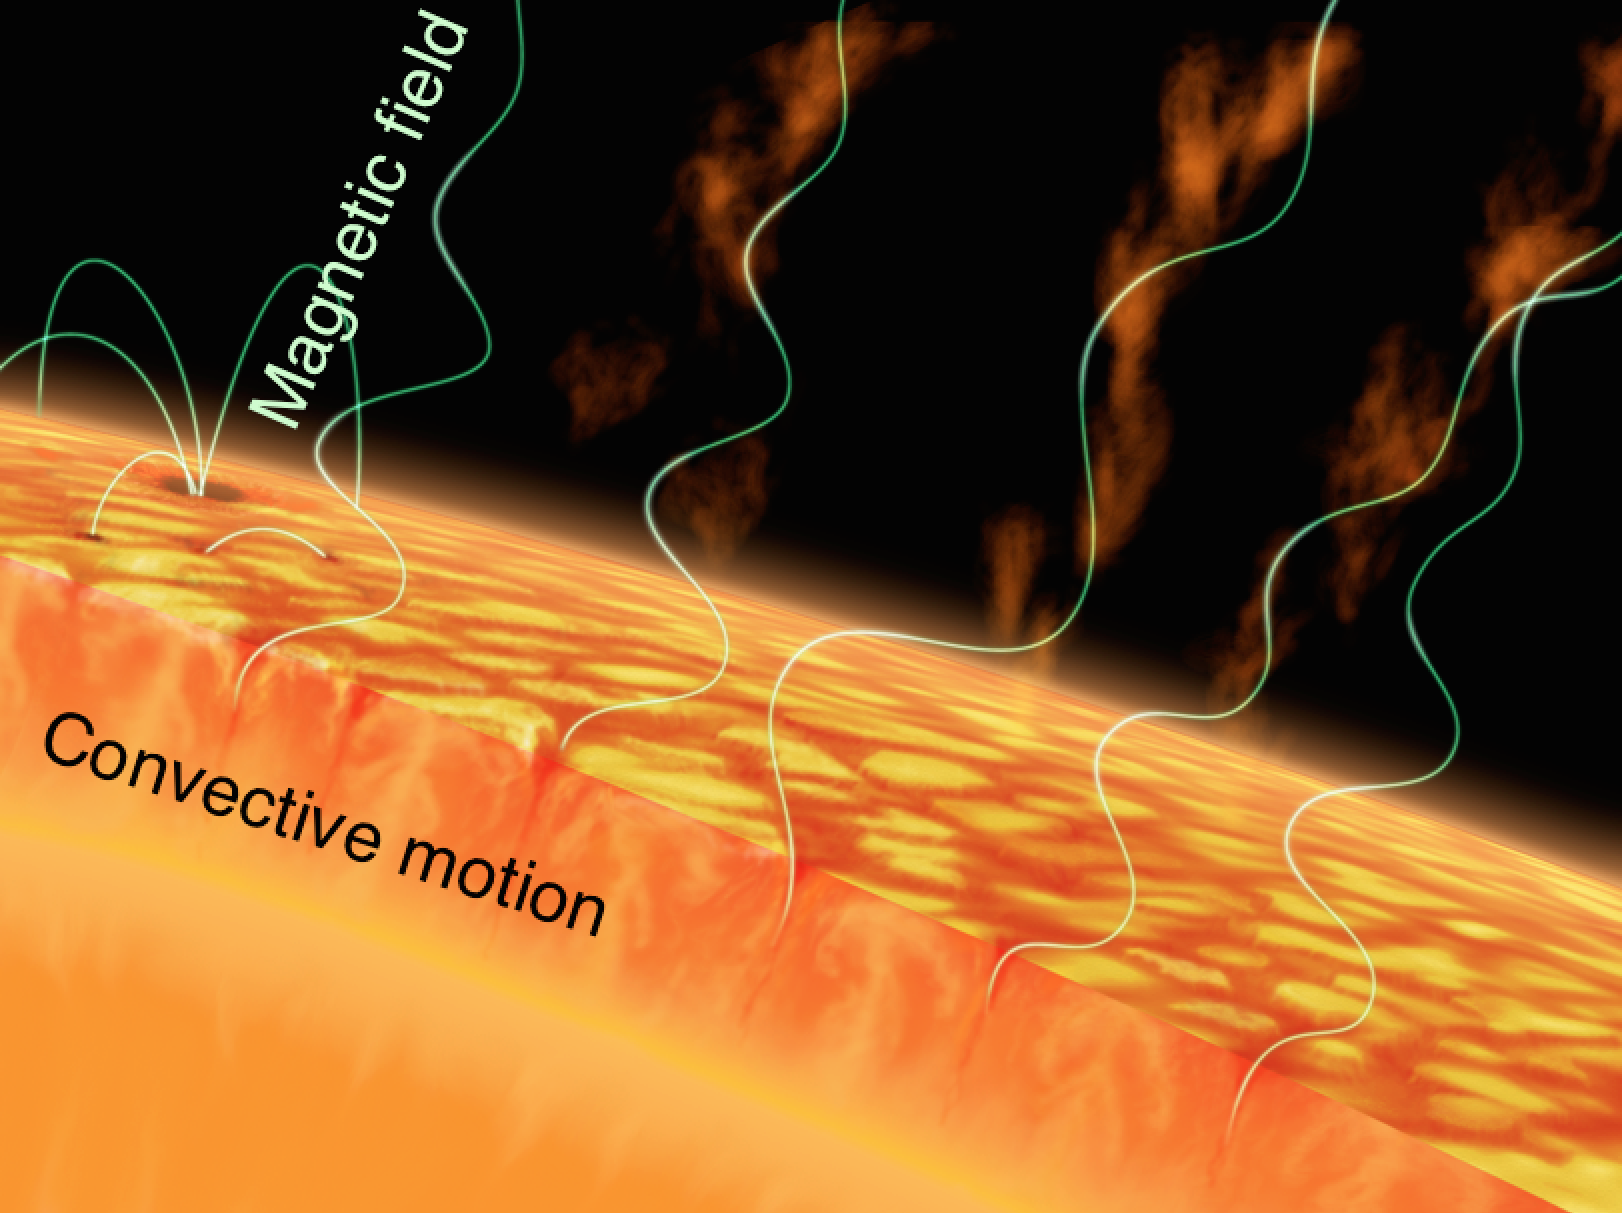
\includegraphics[width=0.95\linewidth]{2023Dundee/Figures/waveheating.png} 
% %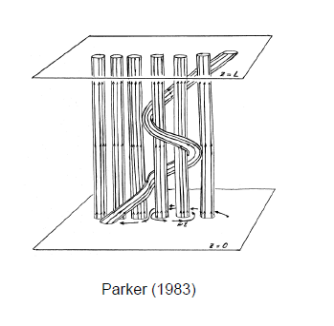
\includegraphics[width=0.95\linewidth]{2023Dundee/Figures/reconnection.png} 
% %Conservative equations (e.g., two-fluid with thermal collisions) leads to MHD shock jumps, Snow \& Hillier 2019.
% %\end{column}
% %\end{columns}
% \end{frame}

% \begin{frame}{Observations}
% \centering
% 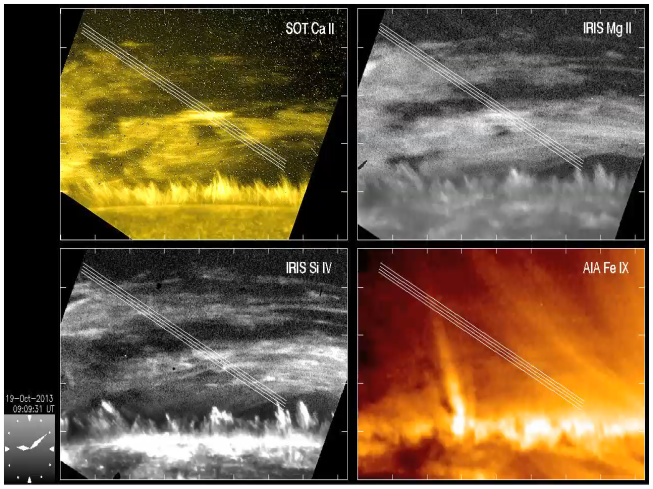
\includegraphics[width=0.75\linewidth]{2023Dundee/Figures/prominence.png}
% \end{frame}

\begin{frame}{Observations}
\centering
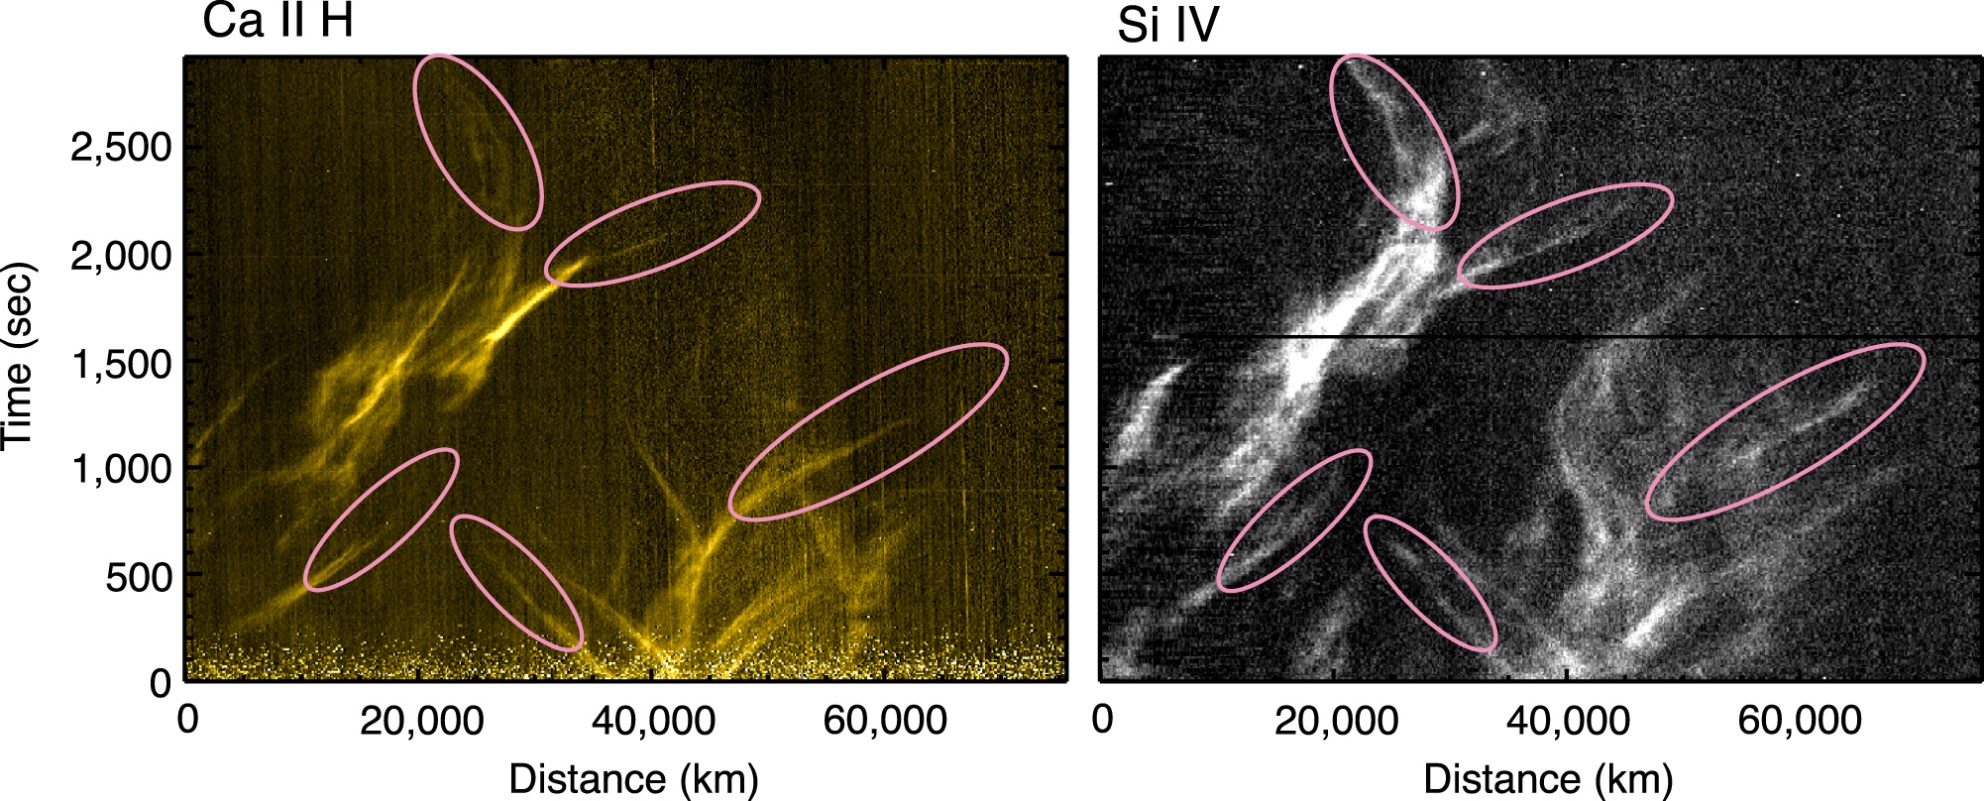
\includegraphics[width=0.95\linewidth]{2023Dundee/Figures/observation.png}
\begin{itemize}
    \item Prominence threads are regularly observed
    \item Cool, dense material embedded in the hot tenuous corona
    \item Seen to fade in cool lines and appear in hotter lines
    \item Heating?
\end{itemize}
\end{frame}

\begin{frame}{Kink-wave $->$ KHI}
%\begin{columns}
%\begin{column}{0.4\textwidth}
%\begin{itemize}
%    \item Theoretical models of this consist of a tube of material that is oscillated
%    \item KHI forms on the edge.
%    \item Turbulent heating?
%    \item Substructure possible.
%\end{itemize}
%\includegraphics[width=1.0\textwidth,clip=true,trim=1.0cm 1.0cm 1.0cm 1.0cm]{obs_shockloc_contour.png}
%\end{column}
%\begin{column}{0.6\textwidth}
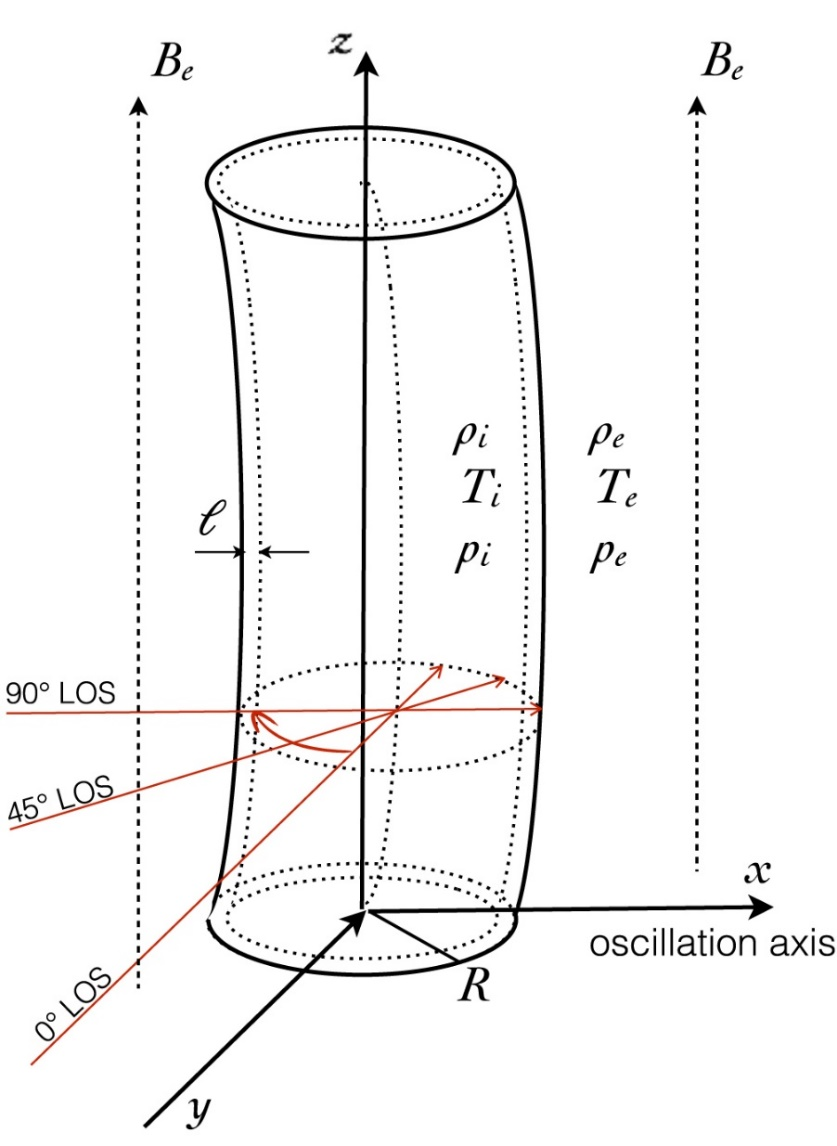
\includegraphics[width=0.35\linewidth]{2023Dundee/Figures/fluxtube.png}
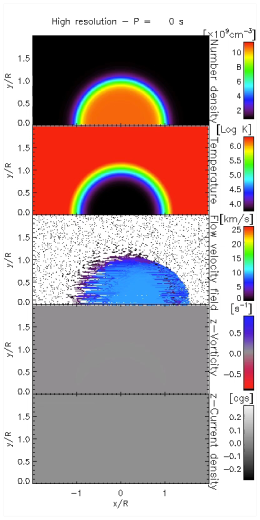
\includegraphics[width=0.3\linewidth]{2023Dundee/Figures/magyarini.png}
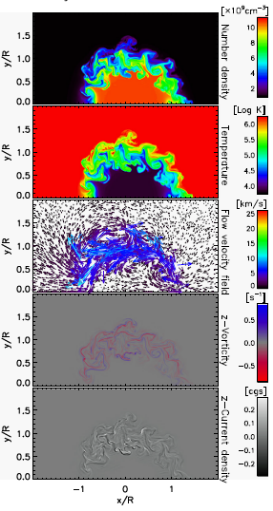
\includegraphics[width=0.3\linewidth]{2023Dundee/Figures/magyarmix.png}
%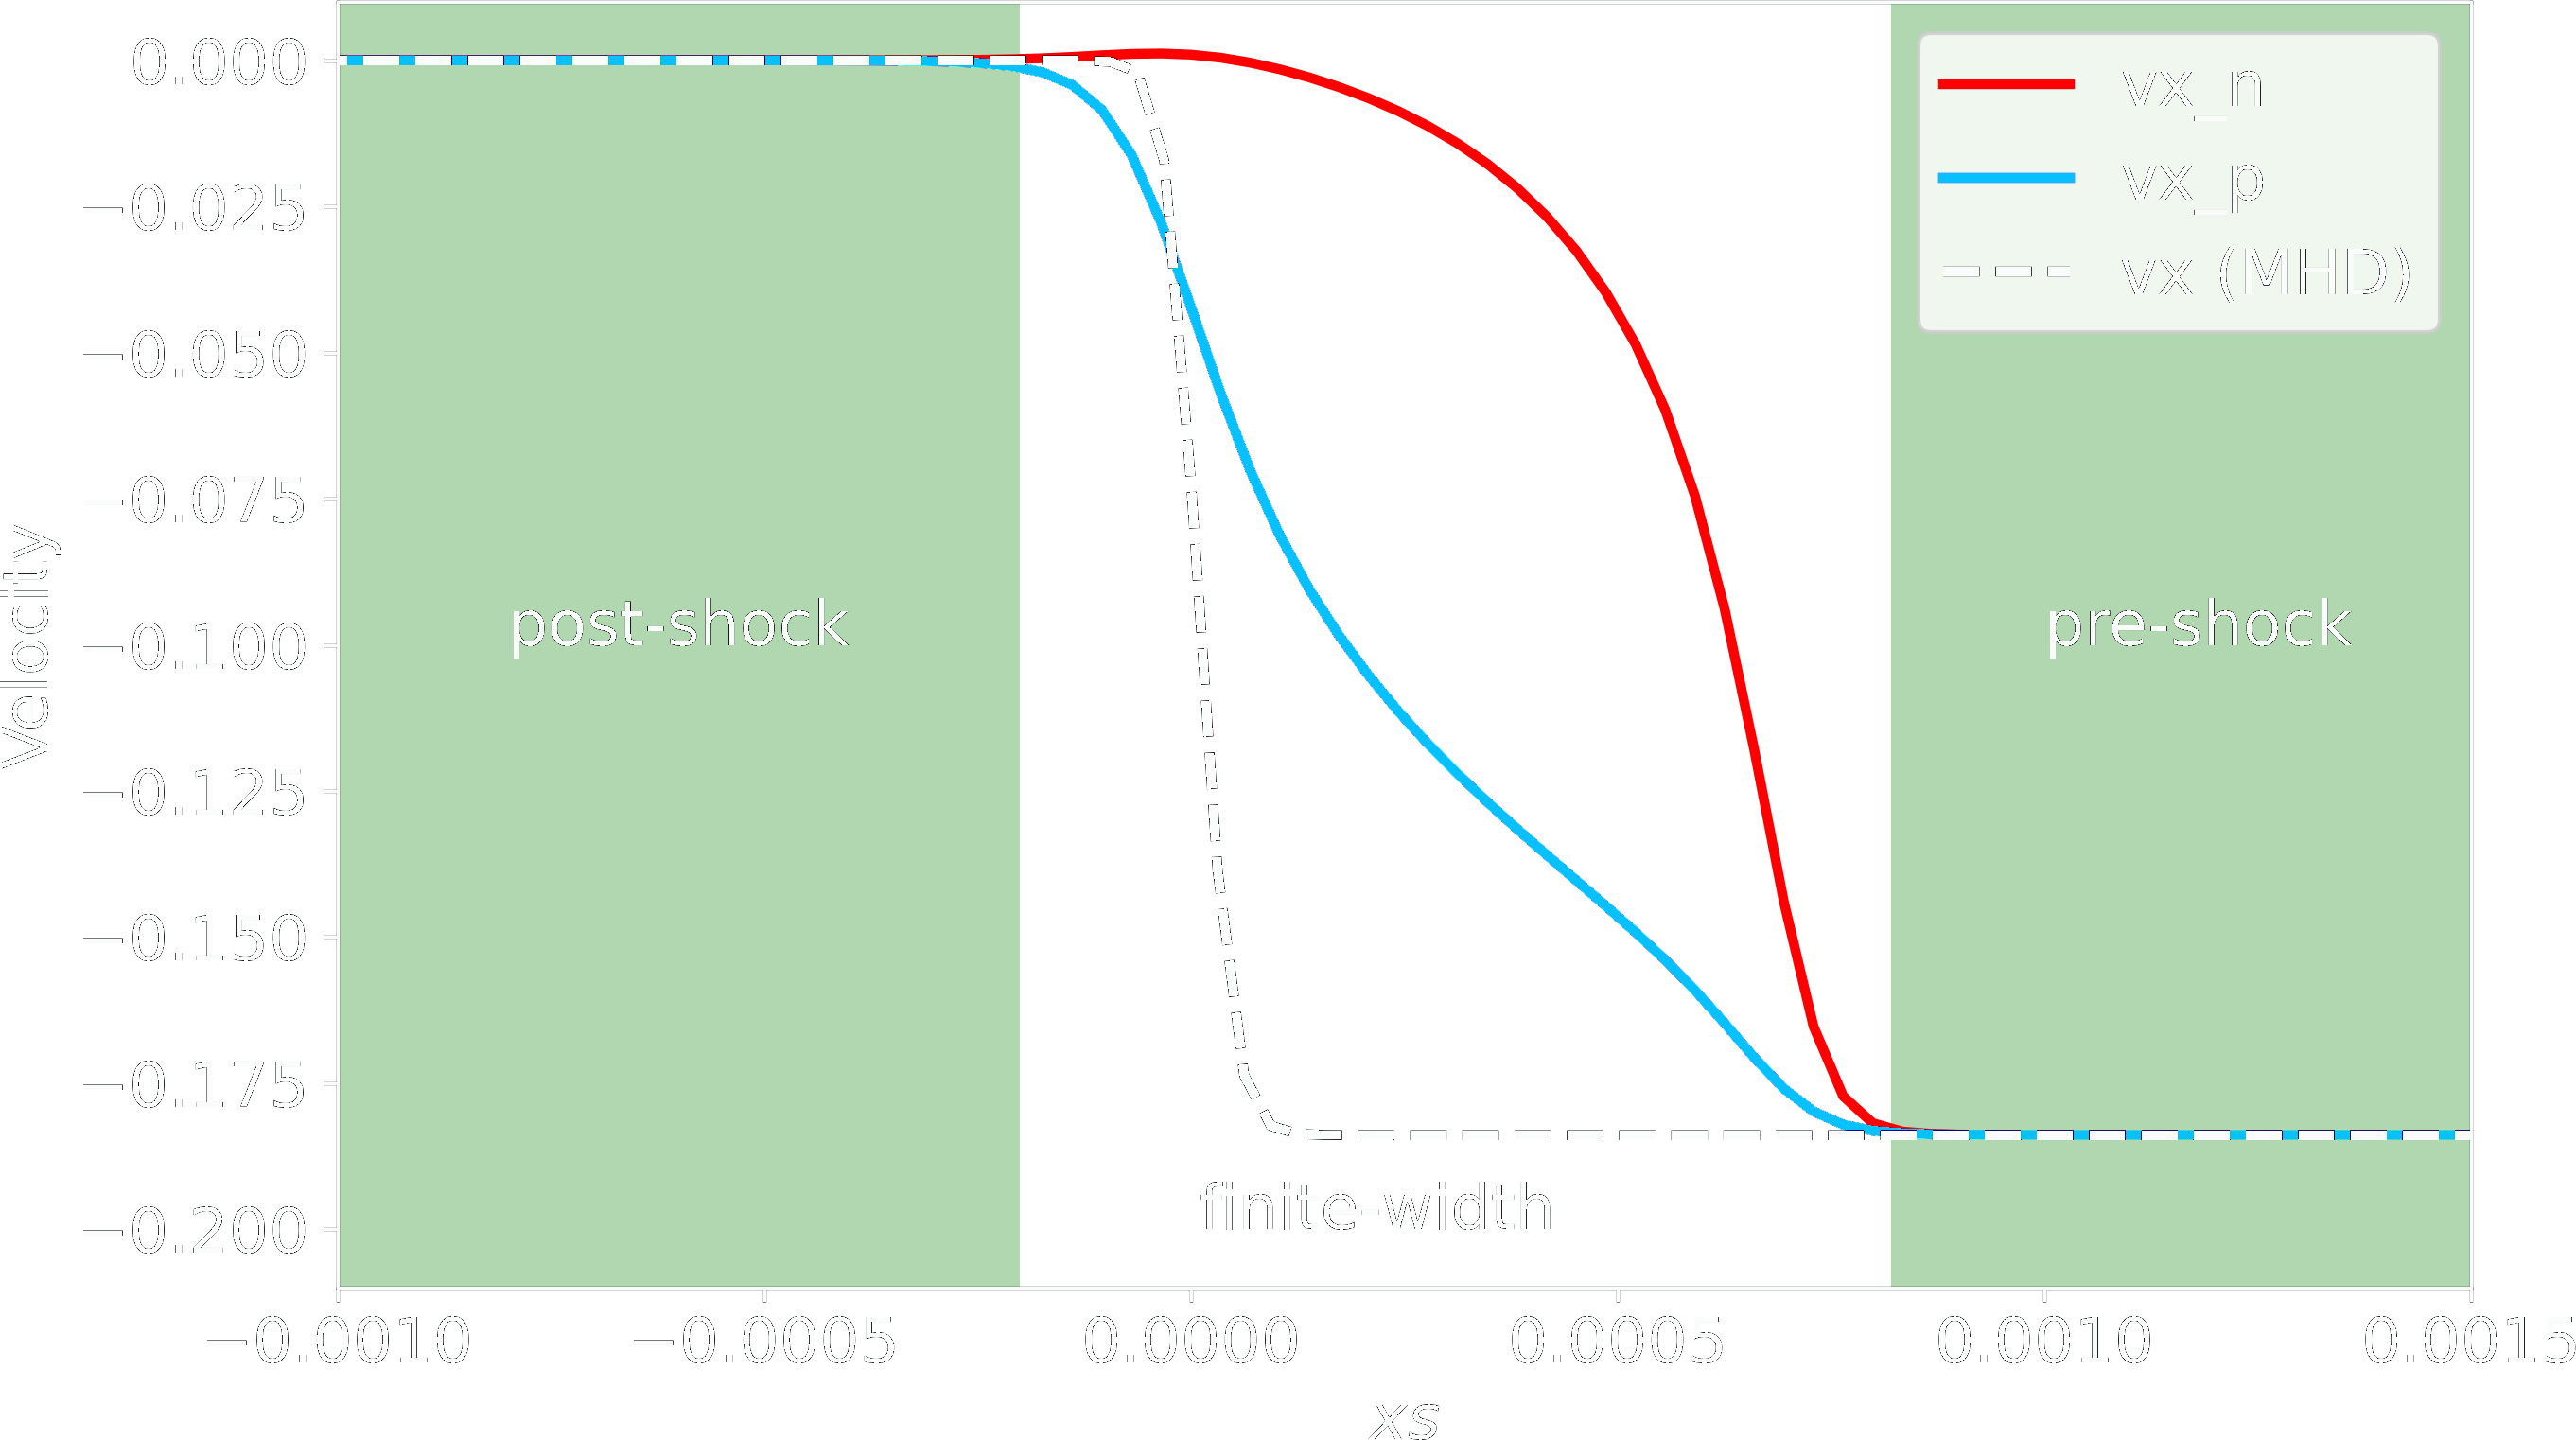
\includegraphics[width=0.95\linewidth]{Figures/shocksub_col.png} \\
%Conservative equations (e.g., two-fluid with thermal collisions) leads to MHD shock jumps, Snow \& Hillier 2019.
%\end{column}
%\end{columns}
\end{frame}


\begin{frame}{Is this really whats going on?}
\begin{columns}
\begin{column}{0.4\textwidth}
\begin{itemize}
    \item Mix hot and cold produces warm 
    \item Warm material has very efficient radiative losses (losses of the form $\rho^2 \Lambda(T)$
    \item Can KHI lead to cooling?
    \item What would the observational signatures look like?
%    \item Substructure possible.
\end{itemize}
%\includegraphics[width=1.0\textwidth,clip=true,trim=1.0cm 1.0cm 1.0cm 1.0cm]{obs_shockloc_contour.png}
\end{column}
\begin{column}{0.6\textwidth}
%\includegraphics[width=0.95\linewidth,clip=true,trim=0.9cm 7.8cm 1.5cm 7.8cm]{poster_comp.pdf} \\
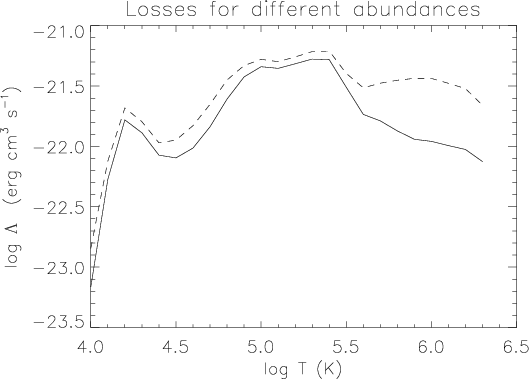
\includegraphics[width=0.95\linewidth]{2023Dundee/Figures/loss.png} \\
%Conservative equations (e.g., two-fluid with thermal collisions) leads to MHD shock jumps, Snow \& Hillier 2019.
\end{column}
\end{columns}
\end{frame}



%%%%%%%%%%%%%%%%%%%%%%%%%%%%%%%%%%%%%%%%%%%%%%%%%%%%%%%%%%%%%%%%%%%%%%%%%%%%%%%%%%

% \begin{frame}{KHI}
% \begin{columns}
% \begin{column}{0.6\textwidth}
% 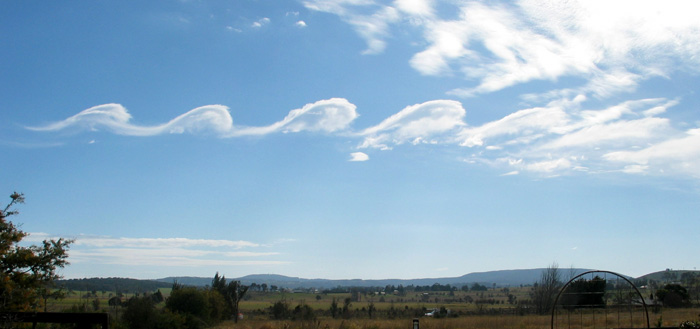
\includegraphics[width=0.95\linewidth]{2023Dundee/Figures/Wavecloudsduval.jpeg} \\
% 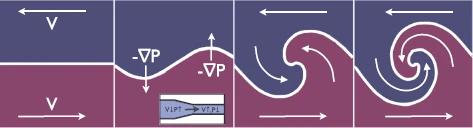
\includegraphics[width=0.95\linewidth]{2023Dundee/Figures/khischematic.png}
% \end{column}
% \begin{column}{0.4\textwidth}
% 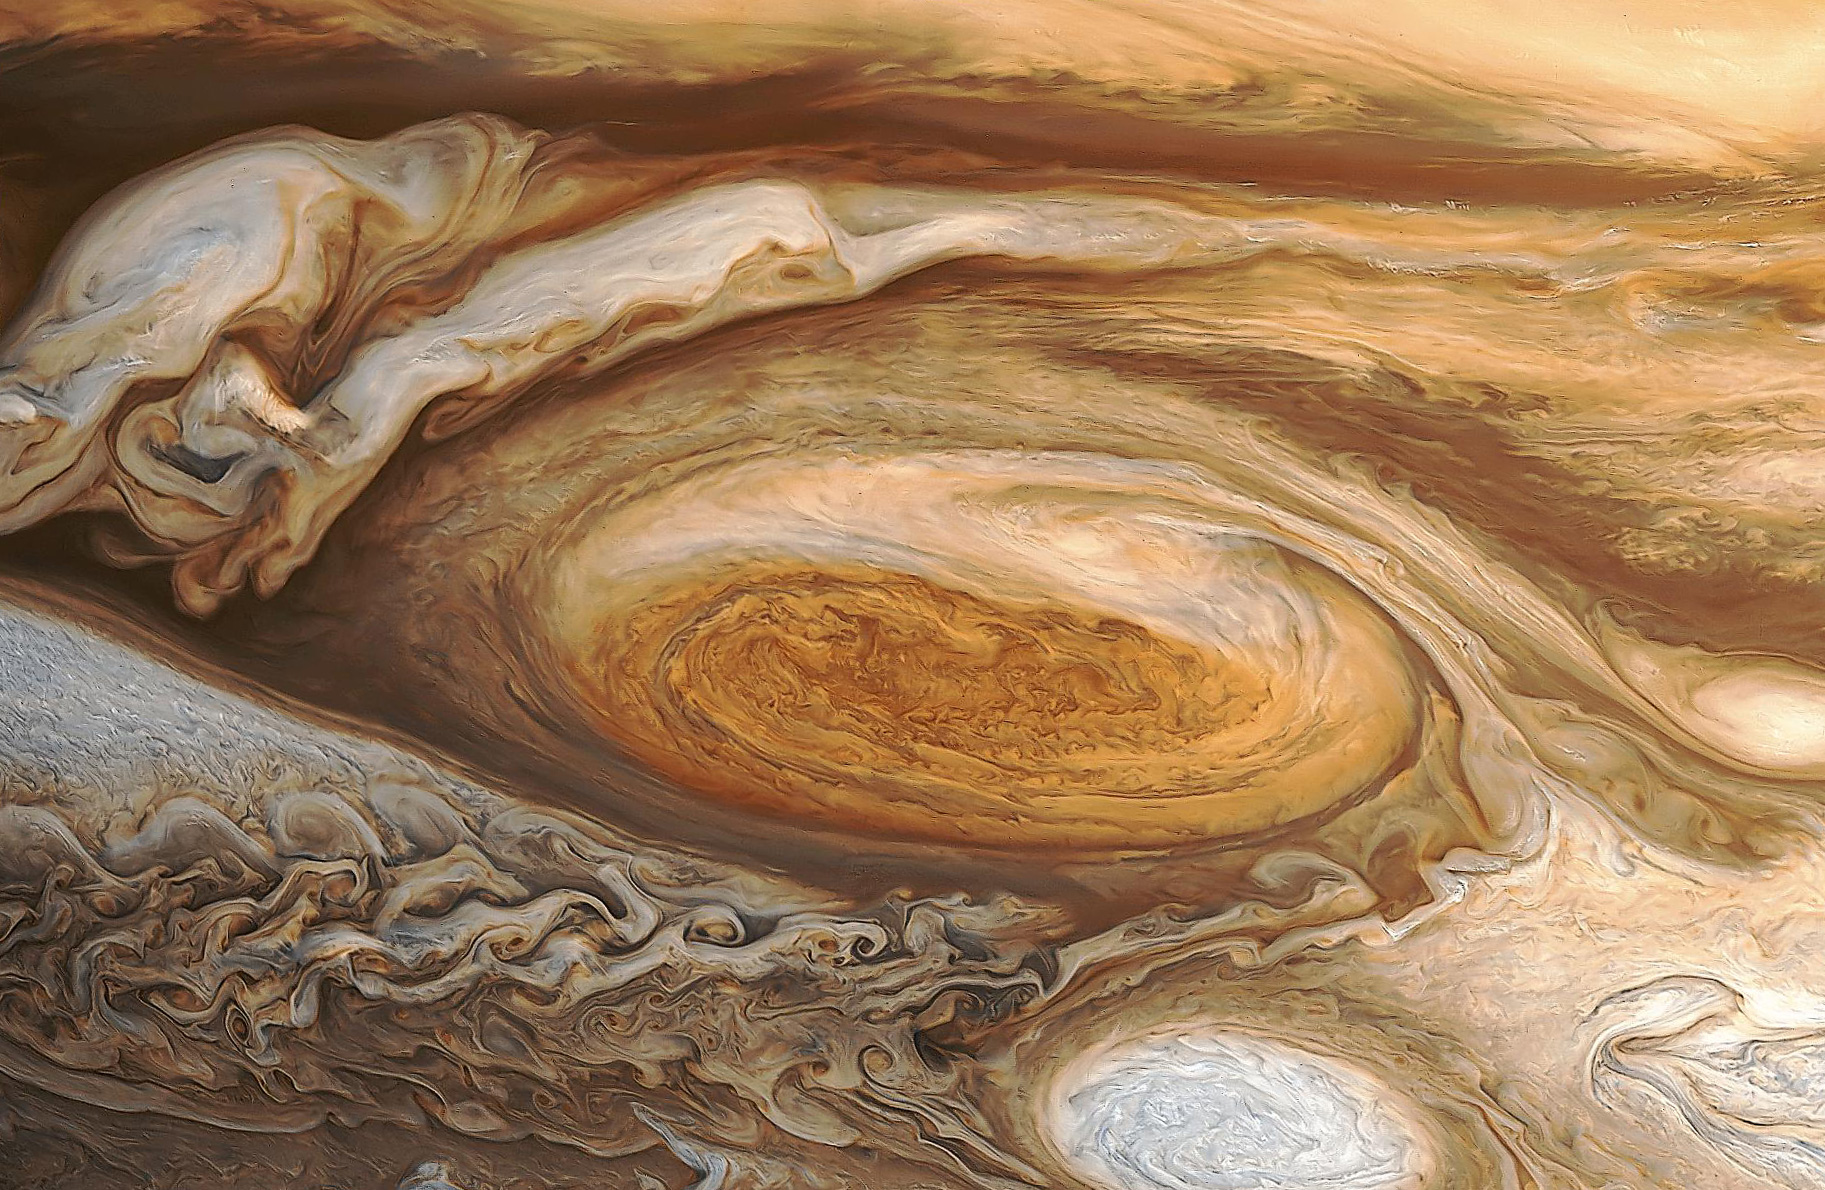
\includegraphics[width=0.95\linewidth]{2023Dundee/Figures/jupiter.png}
% \end{column}
% \end{columns}
% \end{frame}

\begin{frame}{KHI - Analytical approach}
\begin{columns}
\begin{column}{0.4\textwidth}
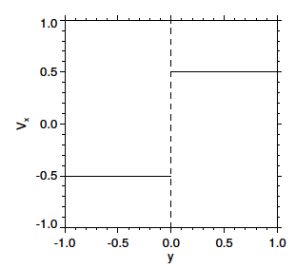
\includegraphics[width=0.95\linewidth]{2023Dundee/Figures/khiinterface.png}
\begin{itemize}
    \item Ideal (HD) KHI evolves in a self-similar way
    \item Width scales according to $W\propto \frac{C_1}{\sqrt(2)} \frac{\left( \rho_1 \rho_2 \right)^{1/4}}{\sqrt{\rho_1}+\sqrt{\rho_2}} \Delta v_t$ (Hillier+2019)
%    \item Substructure possible.
\end{itemize}
%\includegraphics[width=1.0\textwidth,clip=true,trim=1.0cm 1.0cm 1.0cm 1.0cm]{obs_shockloc_contour.png}
\end{column}
\begin{column}{0.6\textwidth}
%\includegraphics[width=0.95\linewidth,clip=true,trim=0.9cm 7.8cm 1.5cm 7.8cm]{poster_comp.pdf} \\
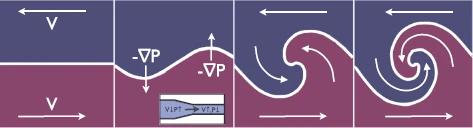
\includegraphics[width=0.95\linewidth]{2023Dundee/Figures/khischematic.png} \\
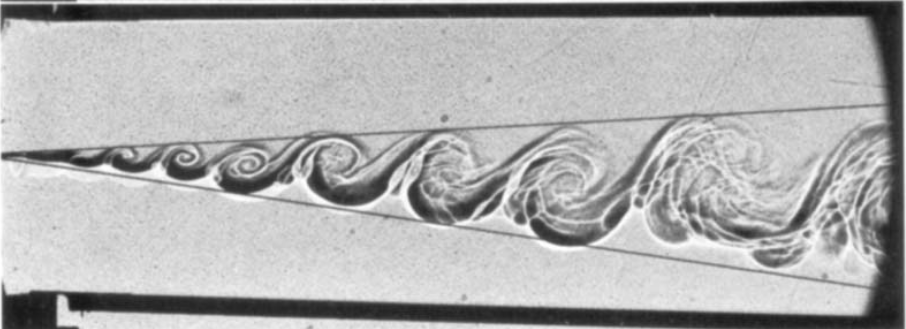
\includegraphics[width=0.95\linewidth]{2023Dundee/Figures/selfsimilar.png} \\
Whole host of assumptions: constant pressure, self-similar, HD evolution, $C_1 \approx 0.5$ empirically determined to match quasi-2D simulations, $T_{mix} \approx \sqrt{T_1 T_2}$
%Conservative equations (e.g., two-fluid with thermal collisions) leads to MHD shock jumps, Snow \& Hillier 2019.
\end{column}
\end{columns}
\end{frame}

% \begin{frame}{Characteristic quantities}
% \begin{columns}
% \begin{column}{0.4\textwidth}
% \begin{itemize}
%     \item Ideal KHI -> self similar
% %    \item Substructure possible.
% \end{itemize}
% %\includegraphics[width=1.0\textwidth,clip=true,trim=1.0cm 1.0cm 1.0cm 1.0cm]{obs_shockloc_contour.png}
% \end{column}
% \begin{column}{0.6\textwidth}
% %\includegraphics[width=0.95\linewidth,clip=true,trim=0.9cm 7.8cm 1.5cm 7.8cm]{poster_comp.pdf} \\
% %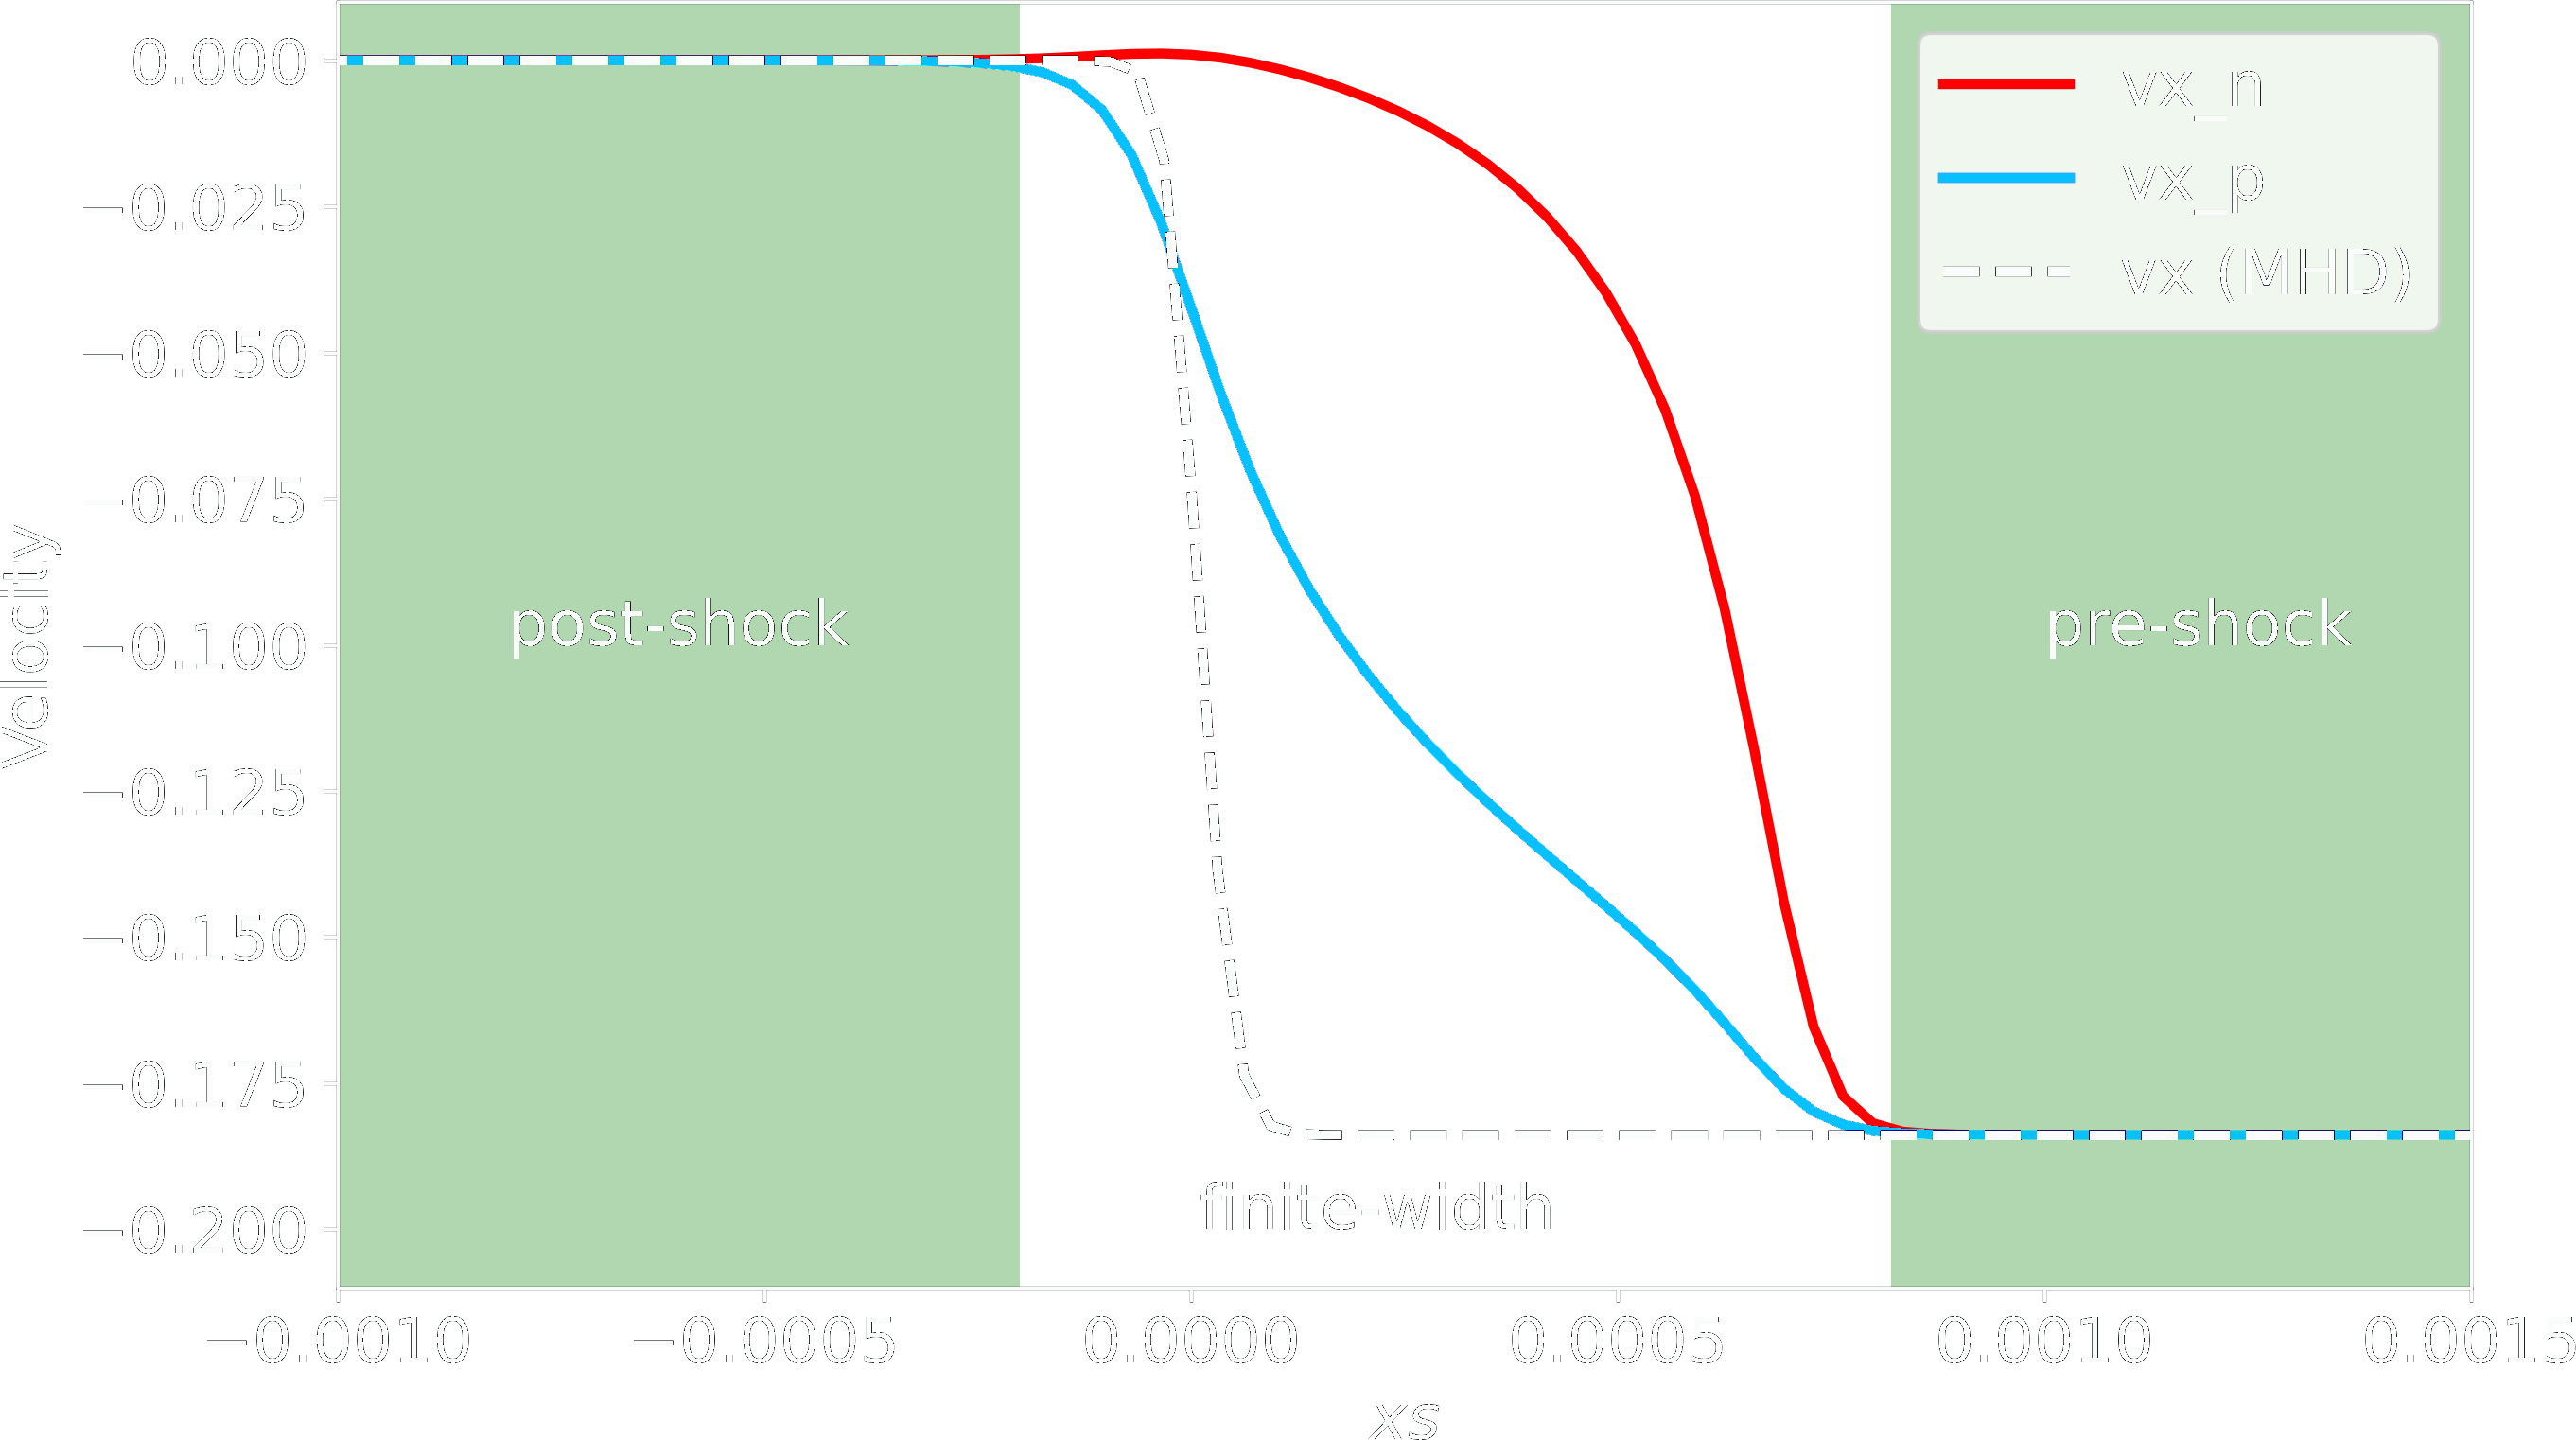
\includegraphics[width=0.95\linewidth]{Figures/shocksub_col.png} \\
% %Conservative equations (e.g., two-fluid with thermal collisions) leads to MHD shock jumps, Snow \& Hillier 2019.
% \end{column}
% \end{columns}
% \end{frame}

\begin{frame}{Cooling induced mixing}
\begin{itemize}
    \item Rate at which thermal energy is brought into the layer
\end{itemize}
\begin{gather}
    \dot{E} \approx \frac{C_1}{\sqrt{2}} L_{mix} D_{mix} \frac{\left( \rho_1 \rho_2 \right)^{1/4}}{\sqrt{\rho_1}+\sqrt{\rho_2}} \Delta v_t \frac{P}{\gamma -1}
\end{gather}
\begin{itemize}
    \item If mixing timescale ($\approx 100$s) is longer than cooling timescale ($\approx 1$s), then mixing is the bottleneck. Therefore, energy is lost at an approximatly constant rate
\end{itemize}
\begin{gather}
    \dot{E}_{loss} \approx \frac{T_{mix}-T_{cut}}{T_{mix}} \dot{E}
\end{gather}
\begin{itemize}
    \item Assumed constant pressure (suitable for the corona where magnetic pressure dominates)
\end{itemize}
\end{frame}

%%%%%%%%%%%%%%%%%%%%%%%%%%%%%%%%%%%%%%%%%%%%%%%%%%%%%%%%%%%%%%%%%%%%%%%%%%%%%%%%%%


\begin{frame}{Numerical model}
\begin{columns}
\begin{column}{0.65\textwidth}
\begin{itemize}
    \item KHI with radiative losses
    \item $\rho_1 =1$, $\rho_2 =100$
    \item Ideal gas law - constant pressure so temperature jumps by 2 orders of magnitude
    \item Magnetic field out of plane (doesn't affect the mixing too much)
    \item Energy removed according to $\rho^2 \Lambda (T)$ using simplified loss equation
\end{itemize}
\end{column}
\begin{column}{0.35\textwidth}
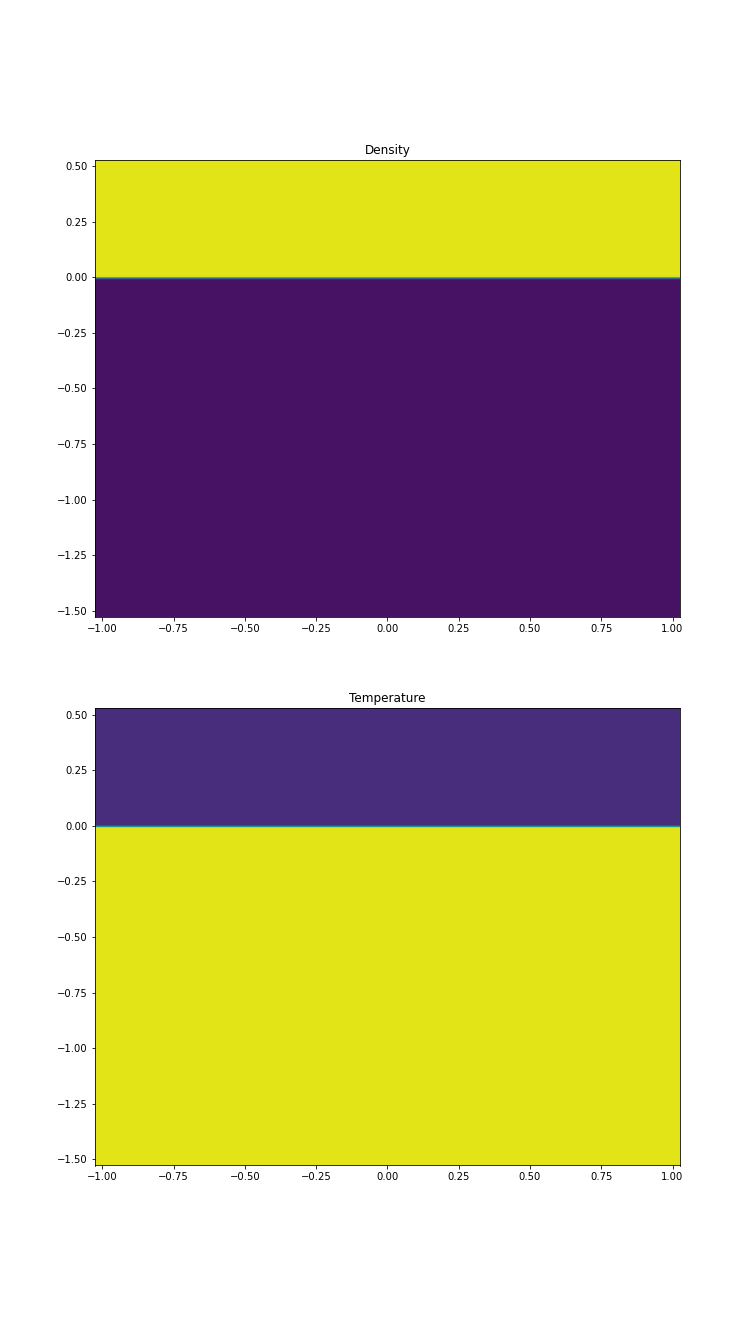
\includegraphics[width=0.95\linewidth]{2023Dundee/Figures/ic.png}
\end{column}
\end{columns}
\end{frame}

\begin{frame}{Loss model}
\begin{columns}
\begin{column}{0.55\textwidth}
\begin{itemize}
    \item Energy removed according to $\rho^2 \Lambda (T)$ using simplified loss equation
    \item tanh type profile centred on $T=10^5$.
    \item Negligible losses in hot and cold regions.
    \item Strong losses in the mixed plasma.
    \item MHD (no losses), $10^5$ (mixing rate$>$loss rate), $10^3$ (mixing rate$\approx$loss rate), $10^1$ (mixing rate$<$loss rate)
\end{itemize}
\end{column}
\begin{column}{0.45\textwidth}
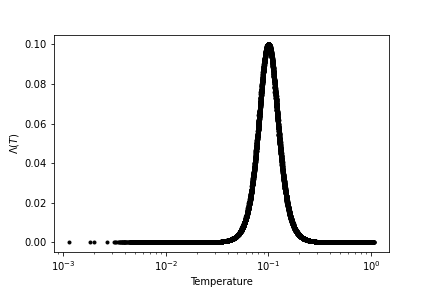
\includegraphics[width=0.95\linewidth]{2023Dundee/Figures/lossprof.png}
\end{column}
\end{columns}
\end{frame}

\begin{frame}{Numerical simulation - density movie}
\end{frame}

\begin{frame}{Numerical simulation - density}
    \centering
   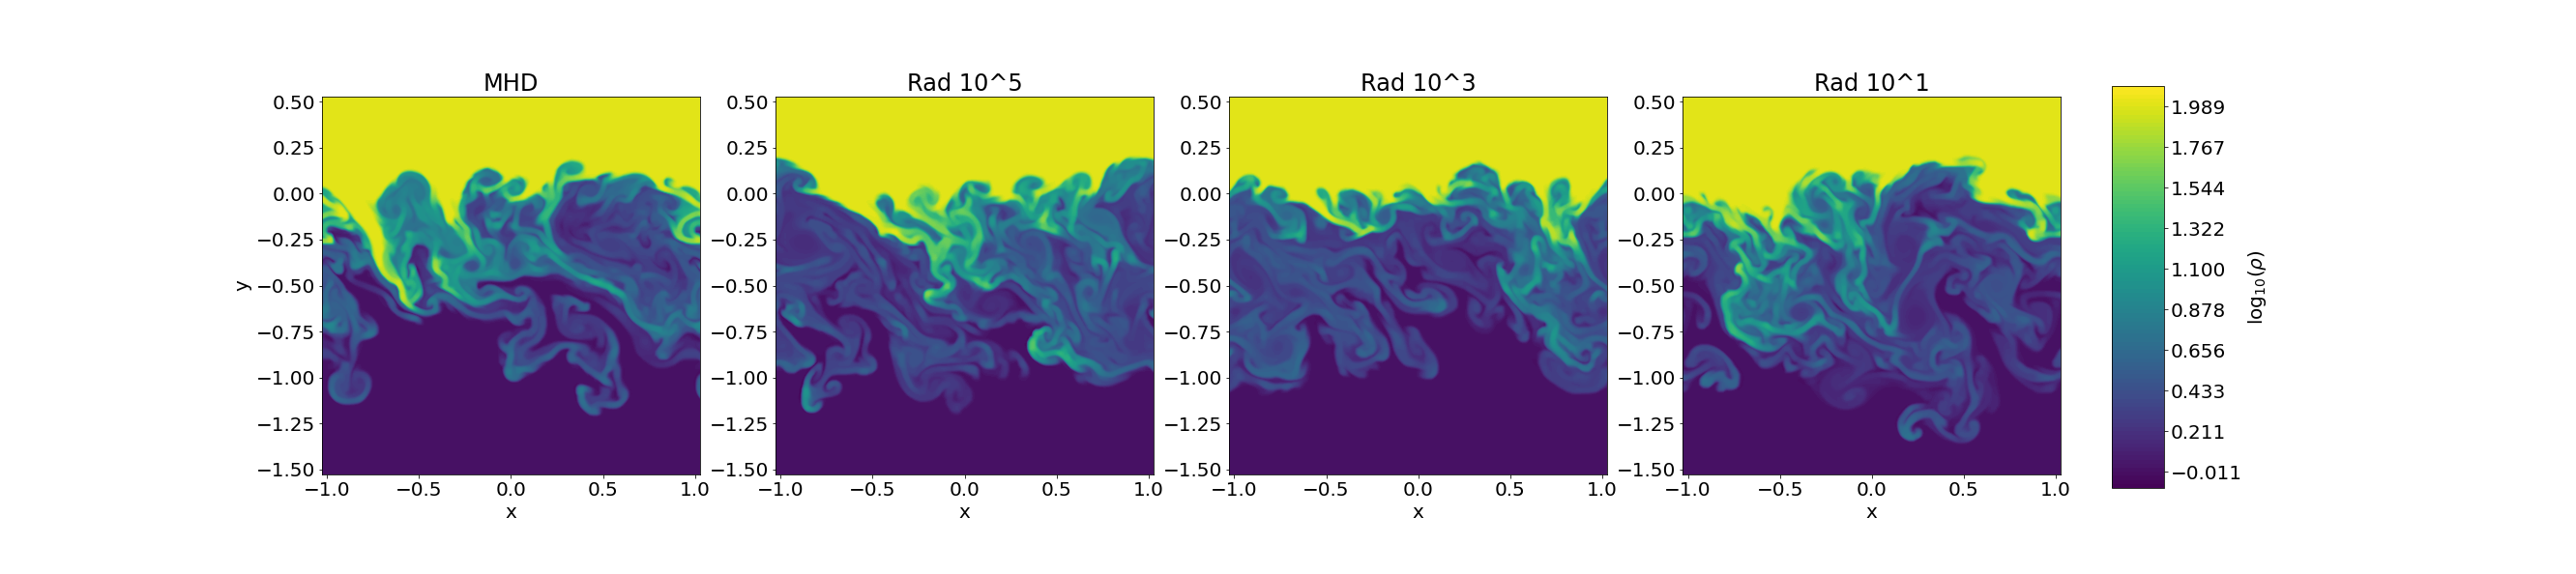
\includegraphics[width=0.99\linewidth,clip=true,trim=7.9cm 0.8cm 8.9cm 0.8cm]{2023Dundee/Figures/denstempevo_rho_t0071.png}
%    \caption{Upper-chromosphere case showing the $v_x$ velocity (top left), $B_y$ magnetic field (top right), temperature (lower left) and density (lower right). For panel c, the reference temperature $T_0=6220$.}
%   \label{fig:upperchromocontext}
%\begin{columns}
%\begin{column}{0.5\textwidth}
%\begin{figure}
    %\centering
%    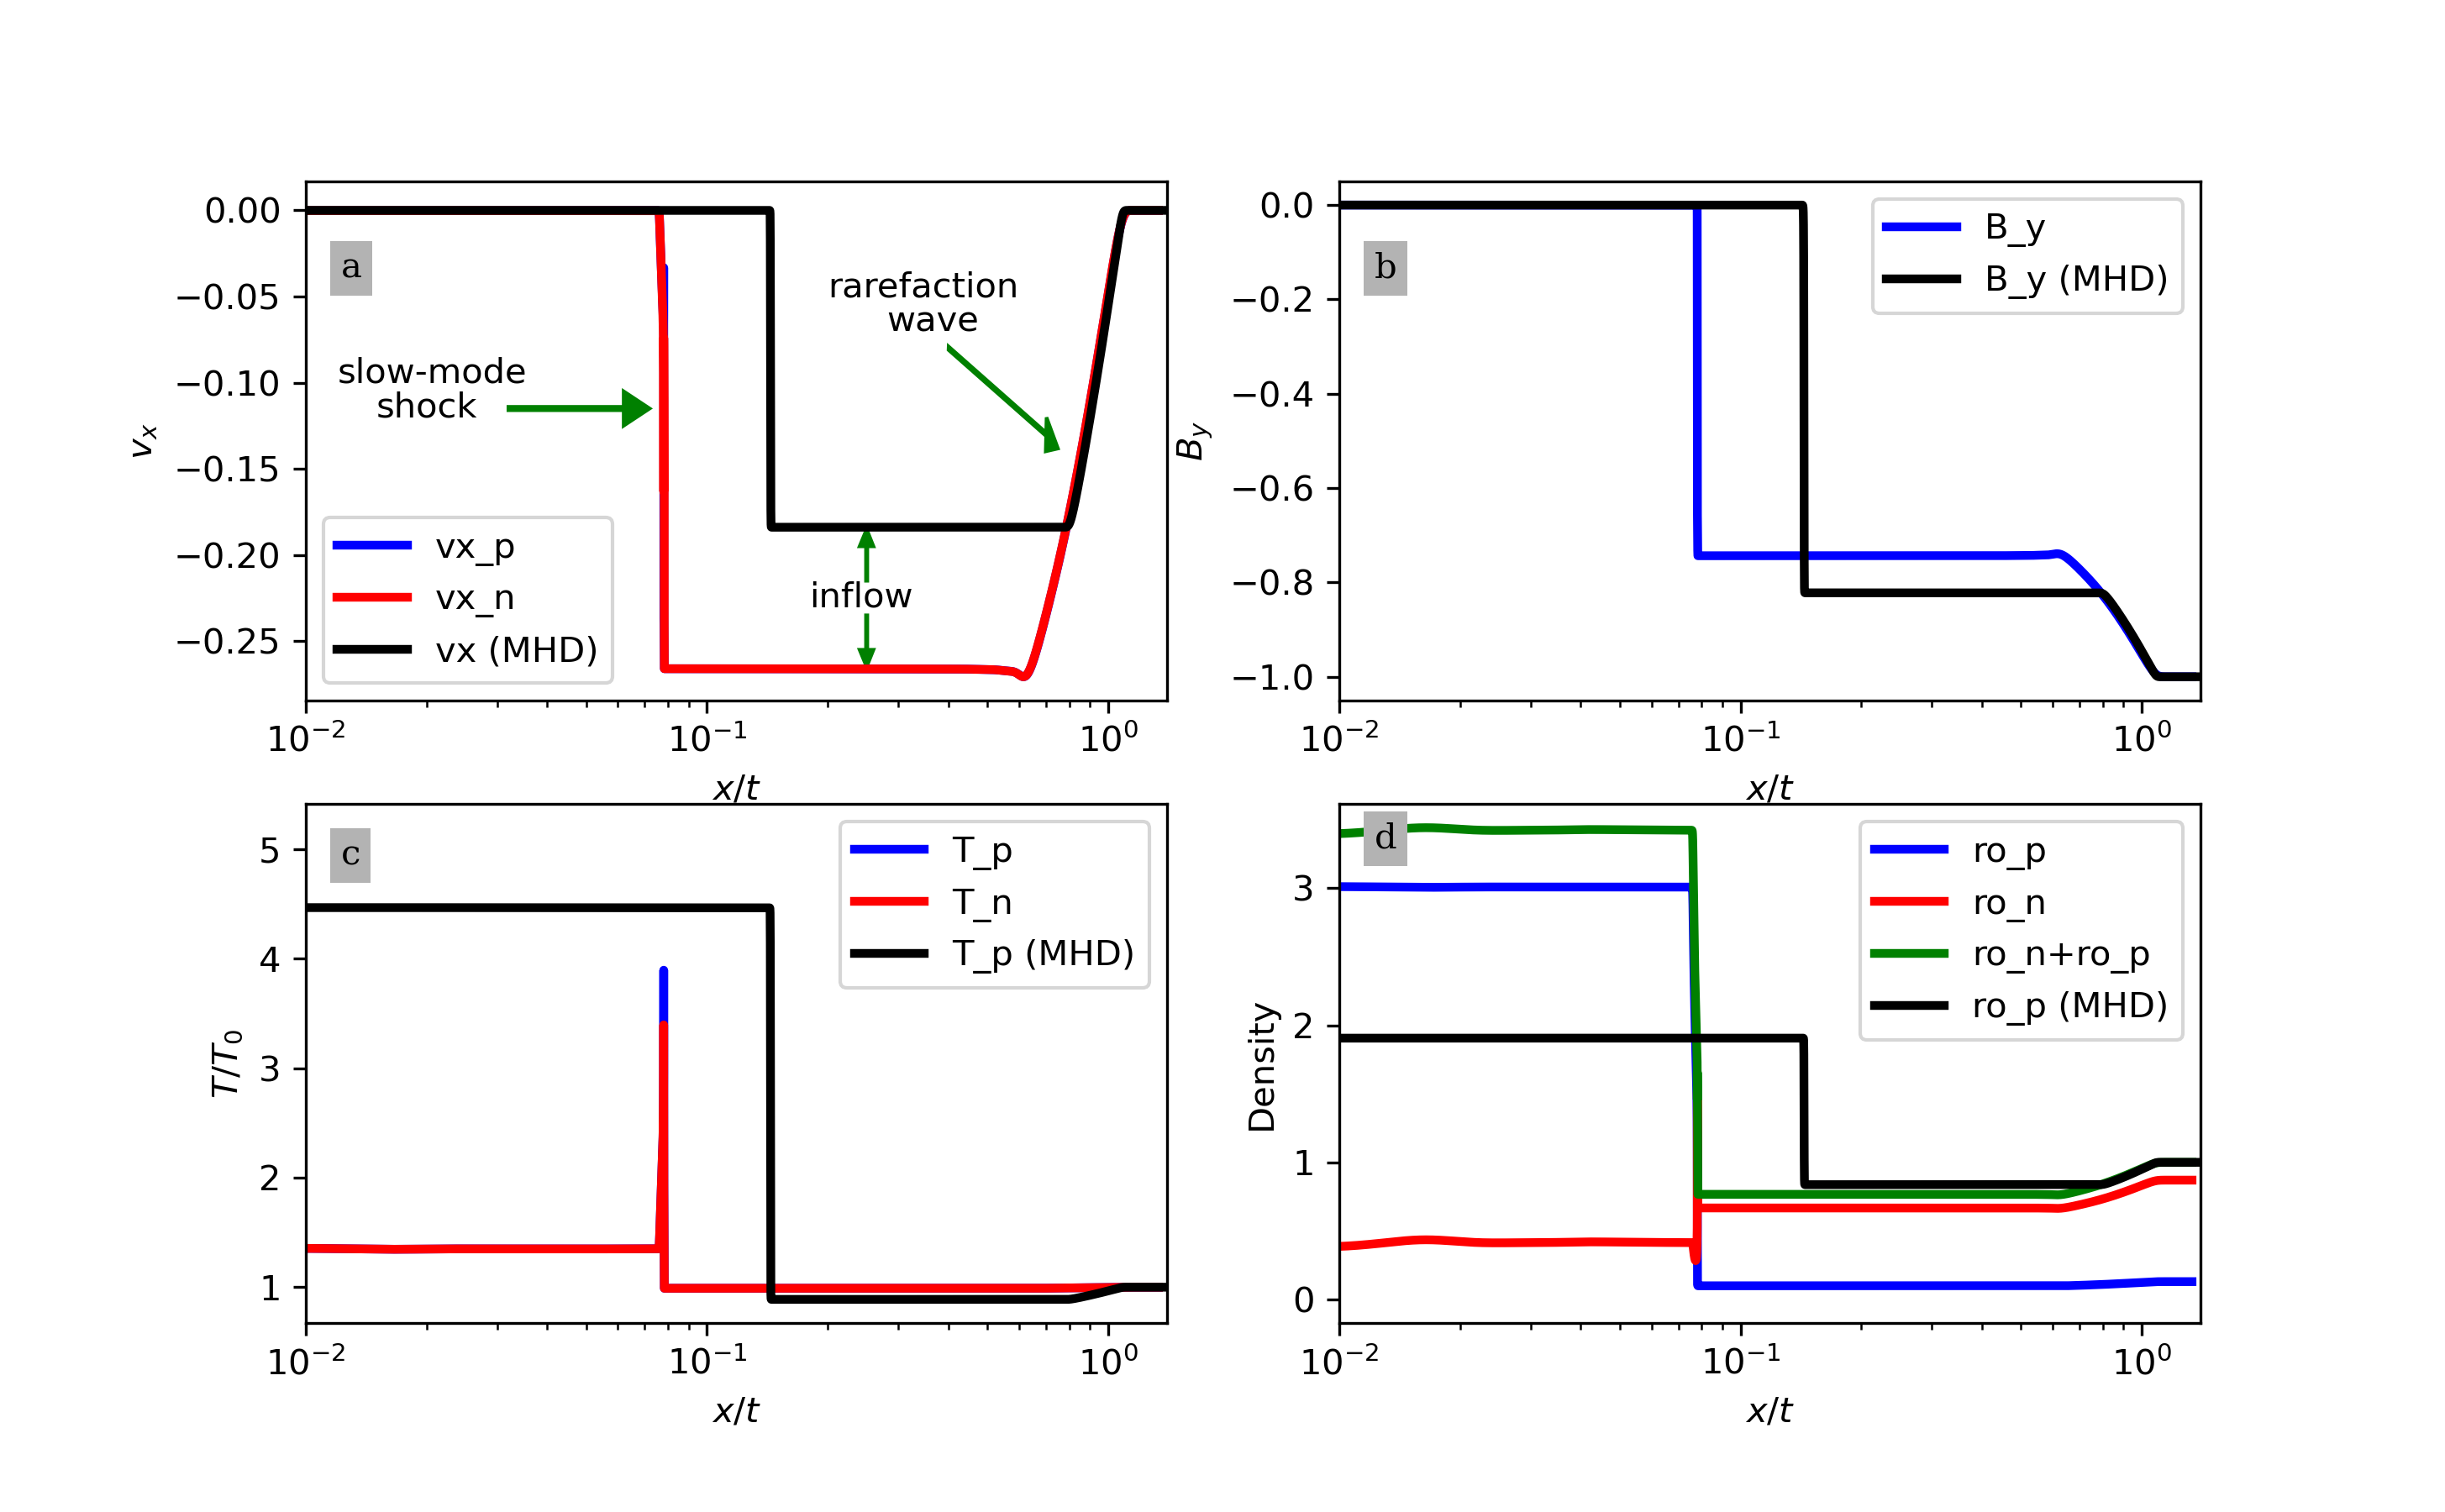
\includegraphics[width=0.95\linewidth,clip=true,trim=0.9cm 0.8cm 0.9cm 0.8cm]{Figures/contextplot.png}
    %\caption{Upper-chromosphere case showing the $v_x$ velocity (top left), $B_y$ magnetic field (top right), temperature (lower left) and density (lower right). For panel c, the reference temperature $T_0=6220$.}
%    \label{fig:upperchromocontext}
%\end{figure}
%\end{column}
%\begin{column}{0.5\textwidth}
%\begin{itemize}
%    $T_0=6220$, $n_e=7.5\times 10^{16}$, $\xi_n=0.87$
%\end{itemize}
\begin{itemize}
    \item No losses on the left. Loss-dominated mixing on the right.
    \item Density looks pretty similar
\end{itemize}
%\end{column}
%\end{columns}
\end{frame}

\begin{frame}{Demonstrate mixing layer fit}
\centering
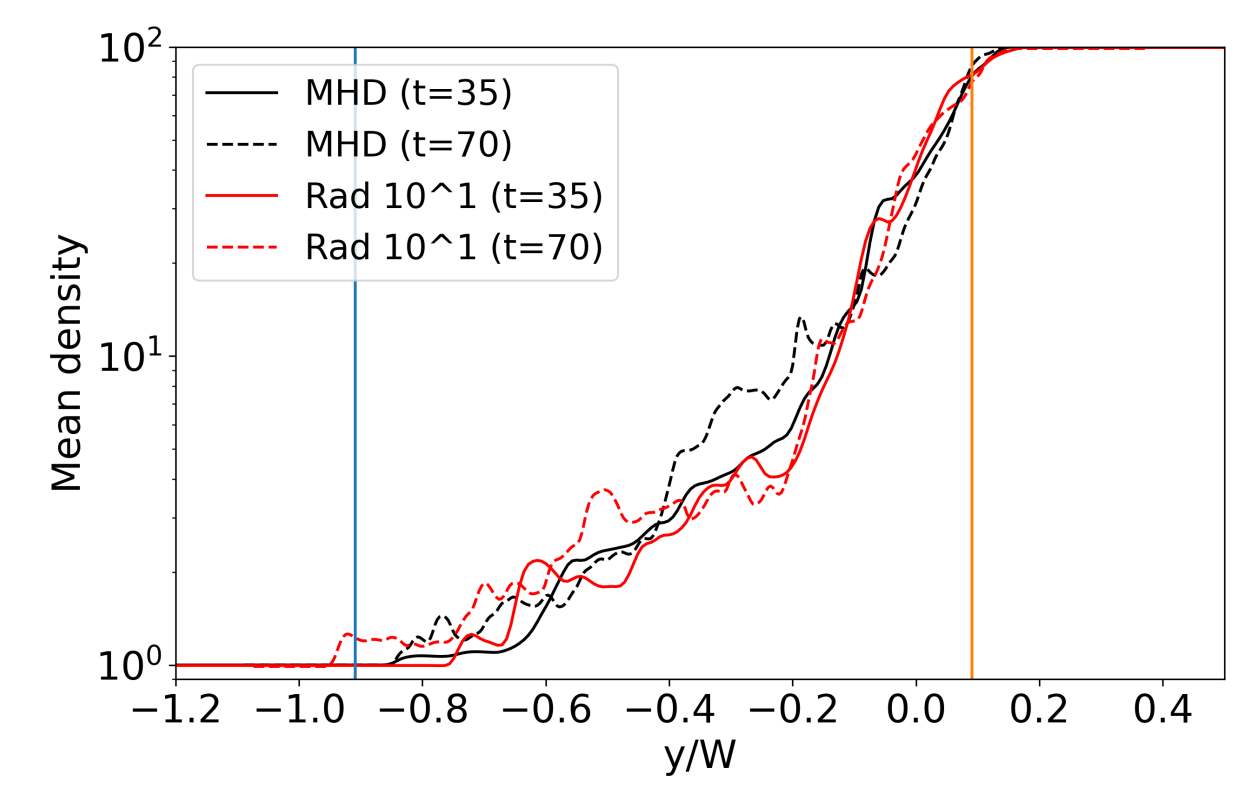
\includegraphics[width=0.85\linewidth]{2023Dundee/Figures/framecheck.png}
\end{frame}

\begin{frame}{Numerical simulation - temperature movie}
\end{frame}

\begin{frame}{Numerical simulation - temperature}
    \centering
   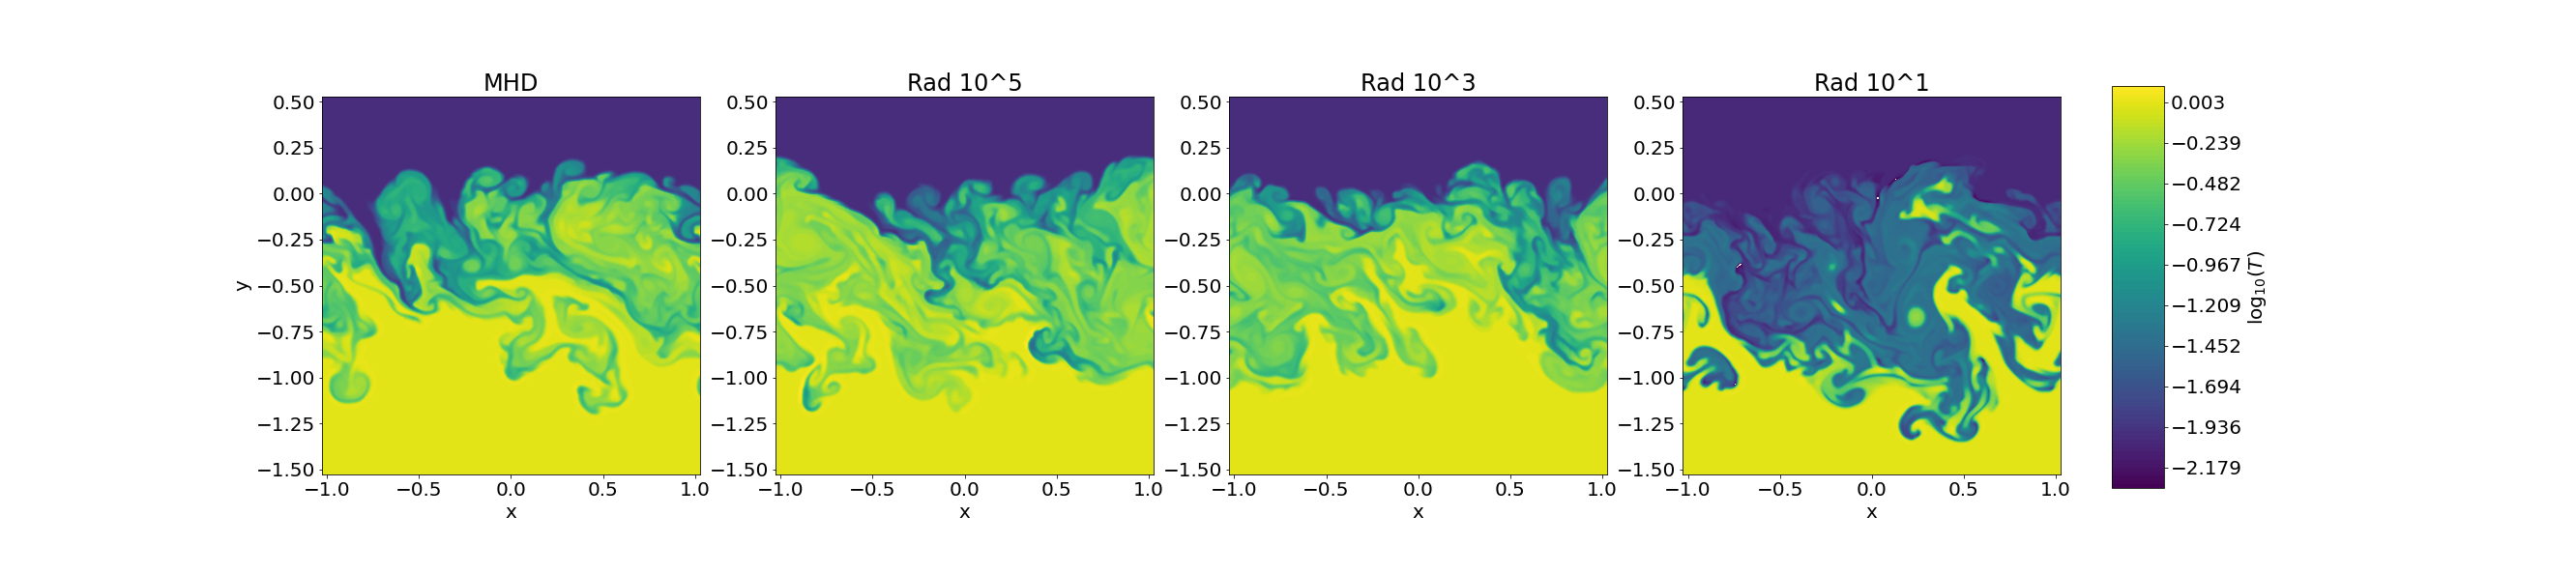
\includegraphics[width=0.99\linewidth,clip=true,trim=7.9cm 0.8cm 8.9cm 0.8cm]{2023Dundee/Figures/denstempevo_T_t0071.png}
\begin{itemize}
    \item Intermediate temperatures not sustained in rapid cooling case
    \item KHI-induced cooling!
\end{itemize}
\end{frame}

\begin{frame}{Predicted cooling rate vs simulations}
\centering
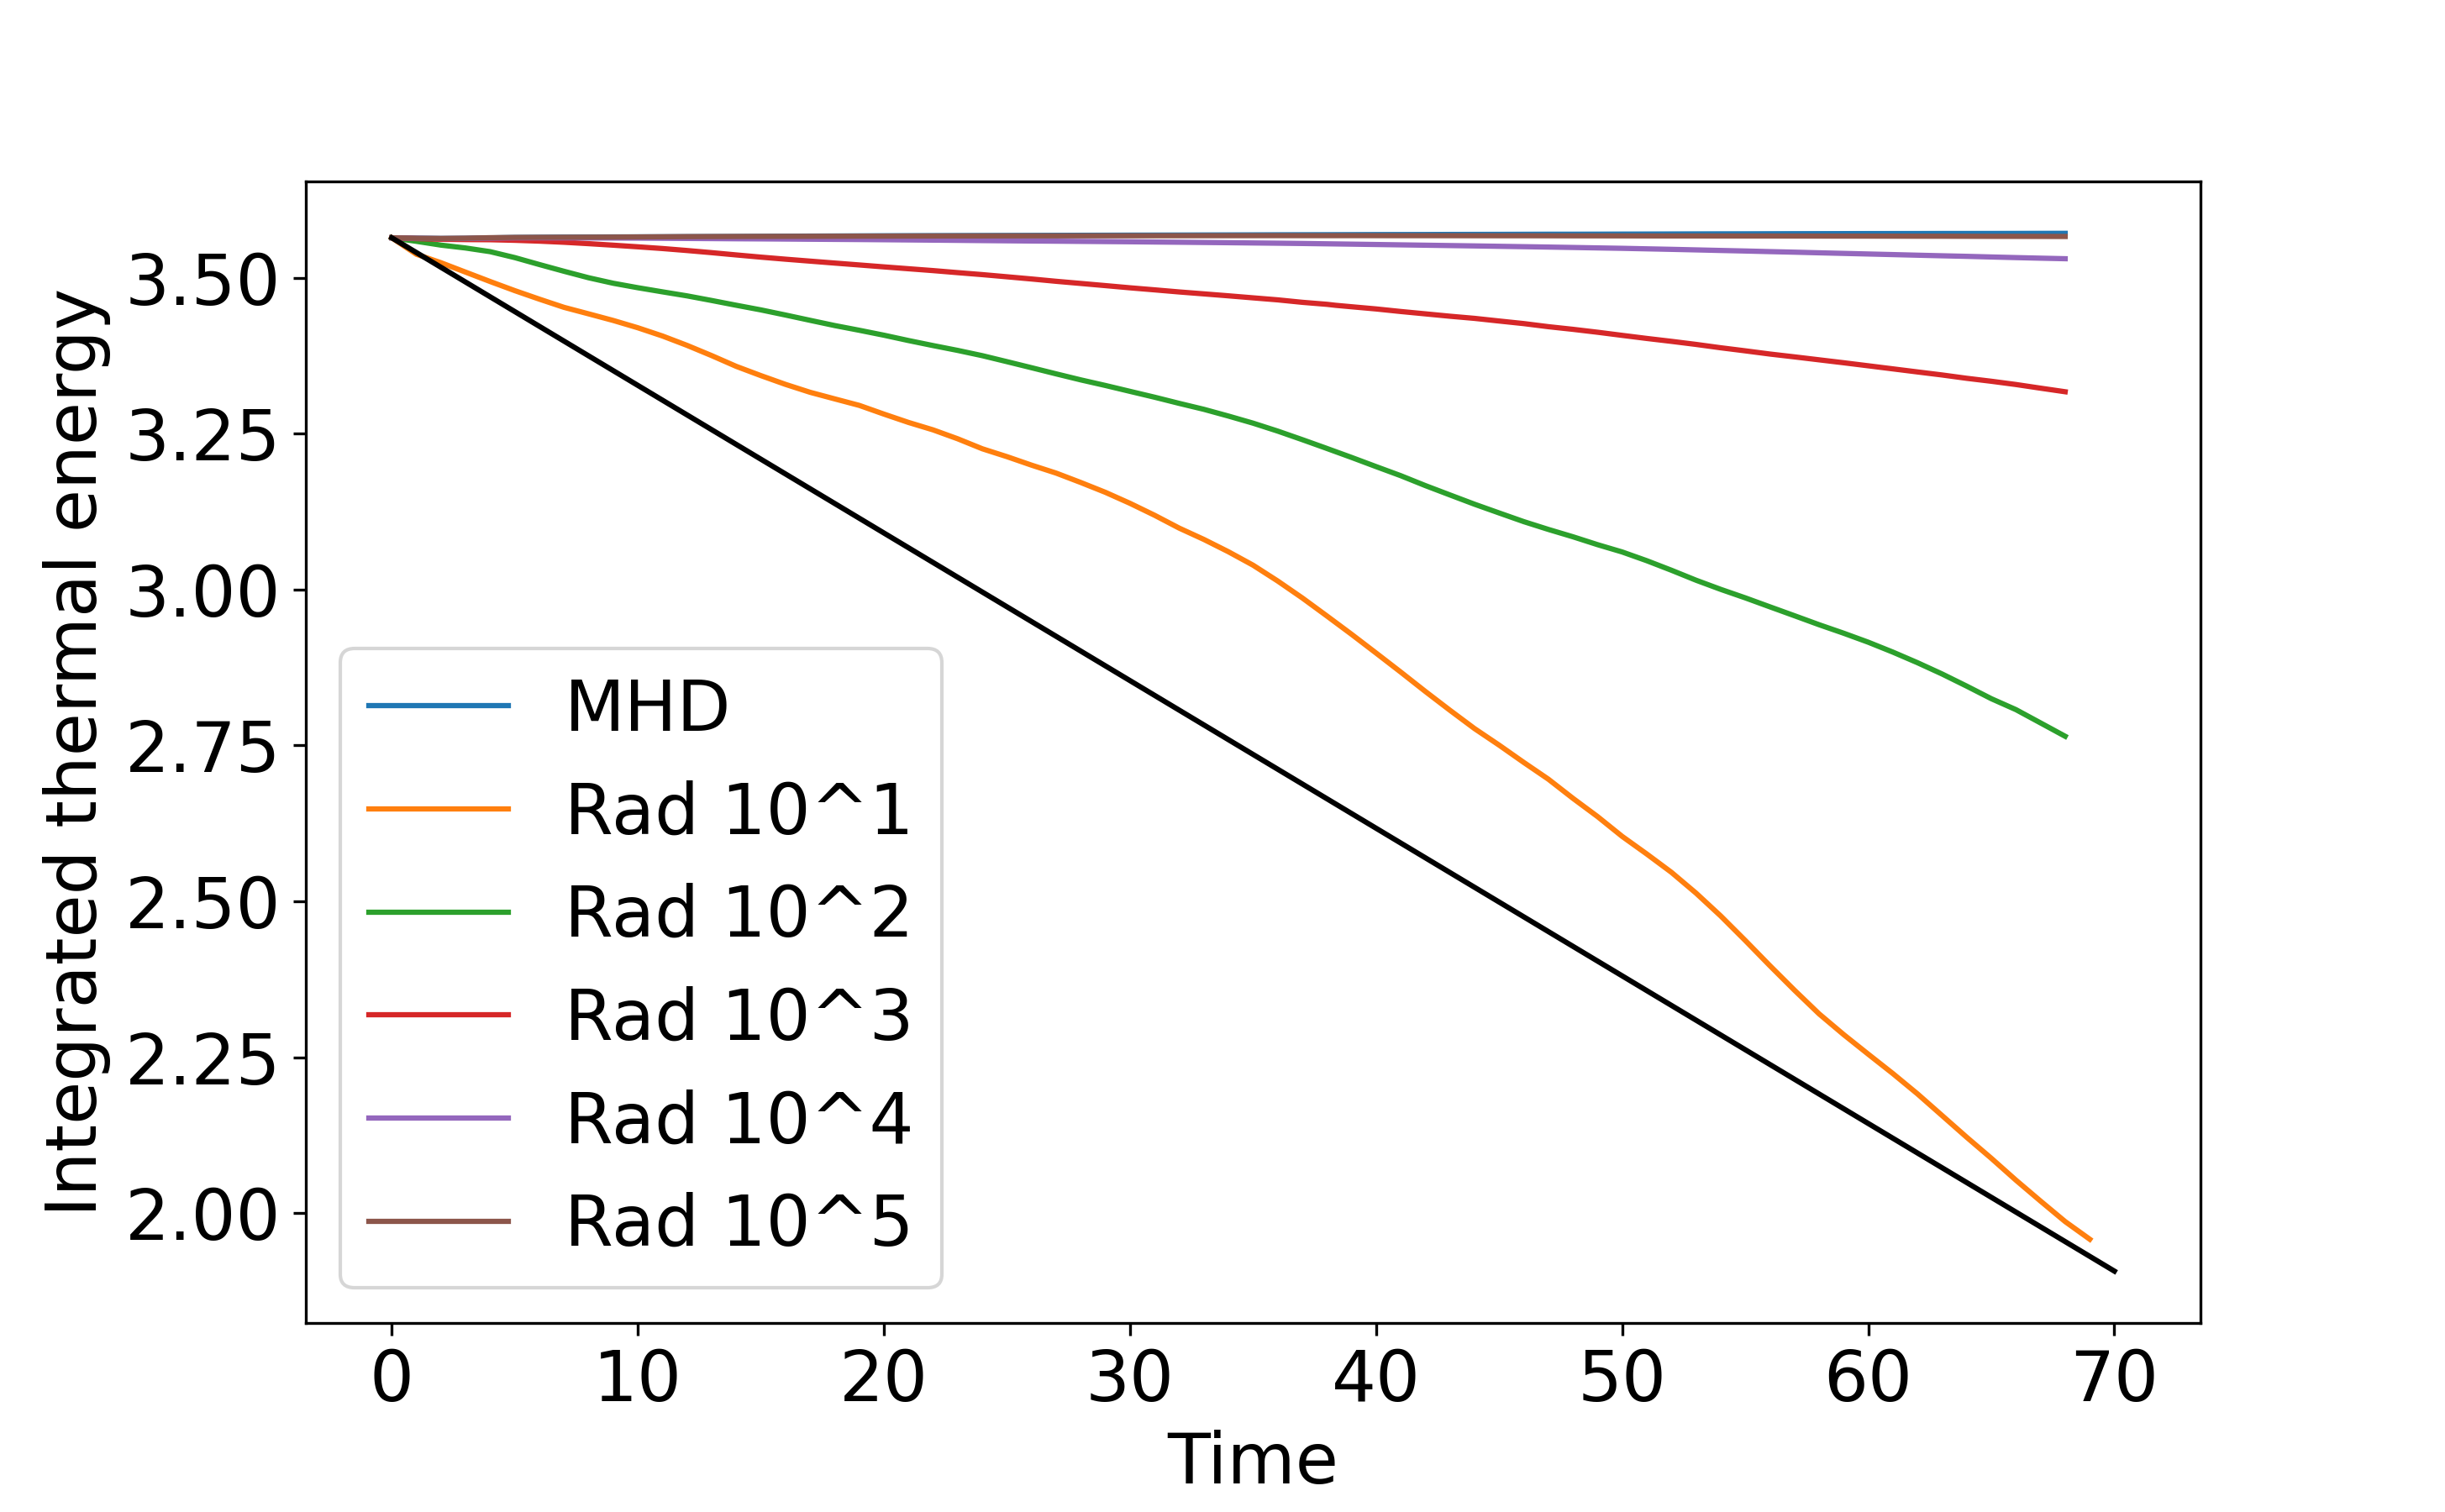
\includegraphics[width=0.85\linewidth,clip=true,trim=0.0cm 0.0cm 0.9cm 0.8cm]{2023Dundee/Figures/integrated_thermal_energy_2.png}
\end{frame}

\begin{frame}{KHI-driven cooling}
\begin{columns}
\begin{column}{0.6\textwidth}
\begin{itemize}
    \item KHI-driven heating assumed to explain observations.
    \item Radiative losses lead to cooling of intermediate temperature that form
    \item KHI-induced cooling!
   % \item But also dense! Dense material leads to more emission. 
   % \item Intensity $\approx \int n_e^2 G(T) dl$
    \item How does this look as an observable? Initially, no emission at $T=10^5$. 
    \item Mixing produces intermediate temperatures and hence emission.
    \item Increased emission in the absence of heating.
\end{itemize}
%\includegraphics[width=1.0\textwidth,clip=true,trim=1.0cm 1.0cm 1.0cm 1.0cm]{obs_shockloc_contour.png}
\end{column}
\begin{column}{0.4\textwidth}
   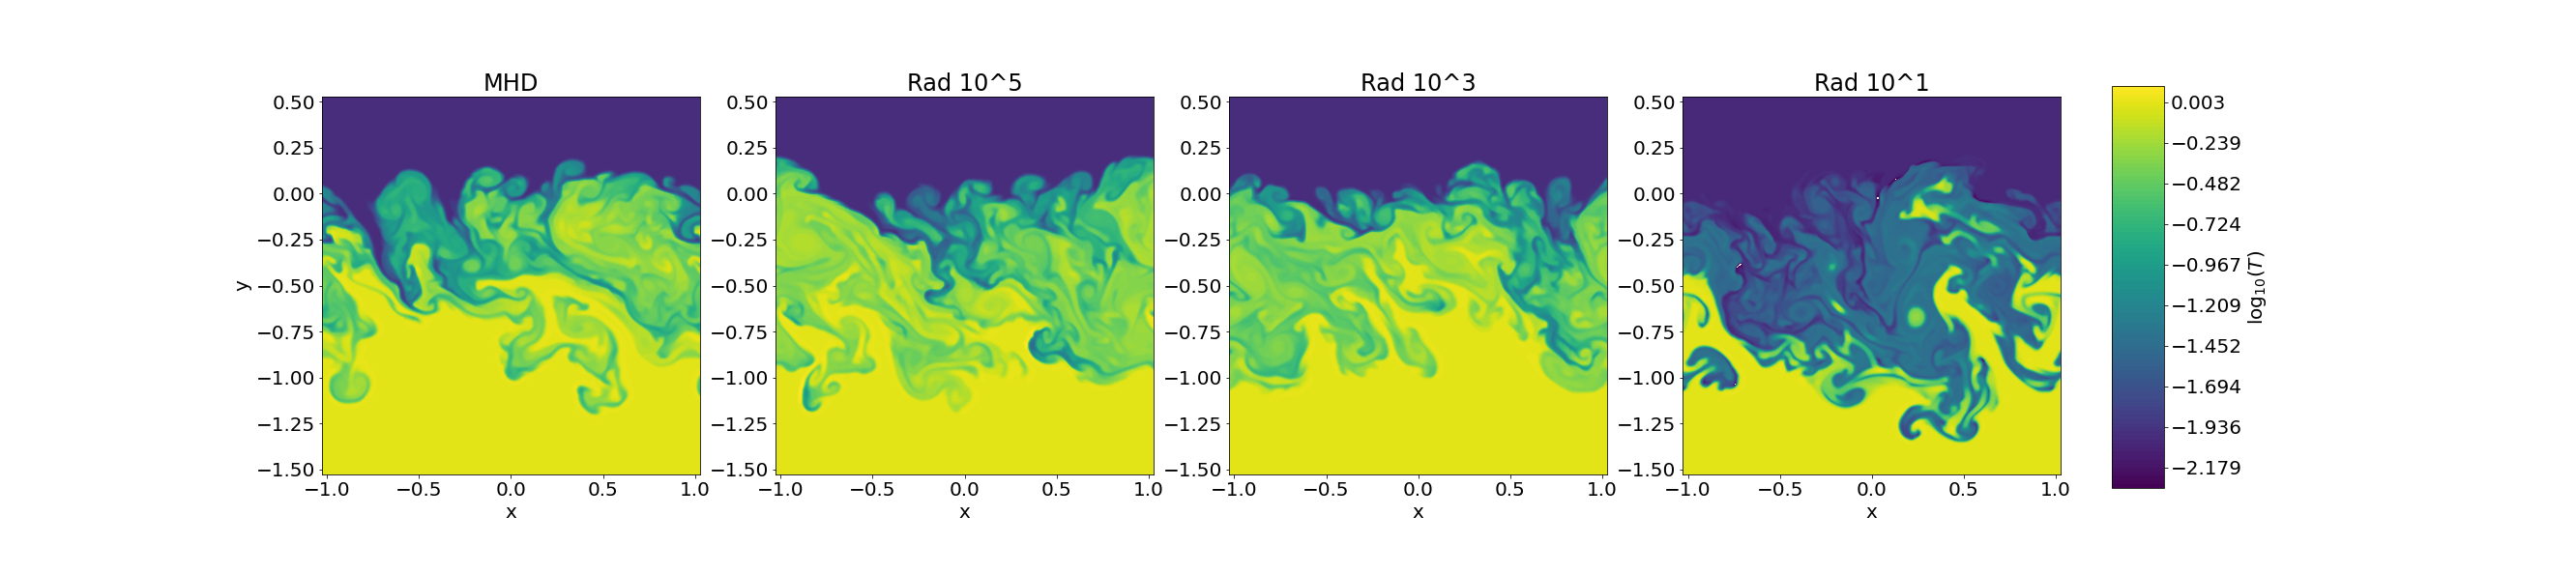
\includegraphics[width=0.99\linewidth,clip=true,trim=58.9cm 0.8cm 8.9cm 0.8cm]{2023Dundee/Figures/denstempevo_T_t0071.png} \\
   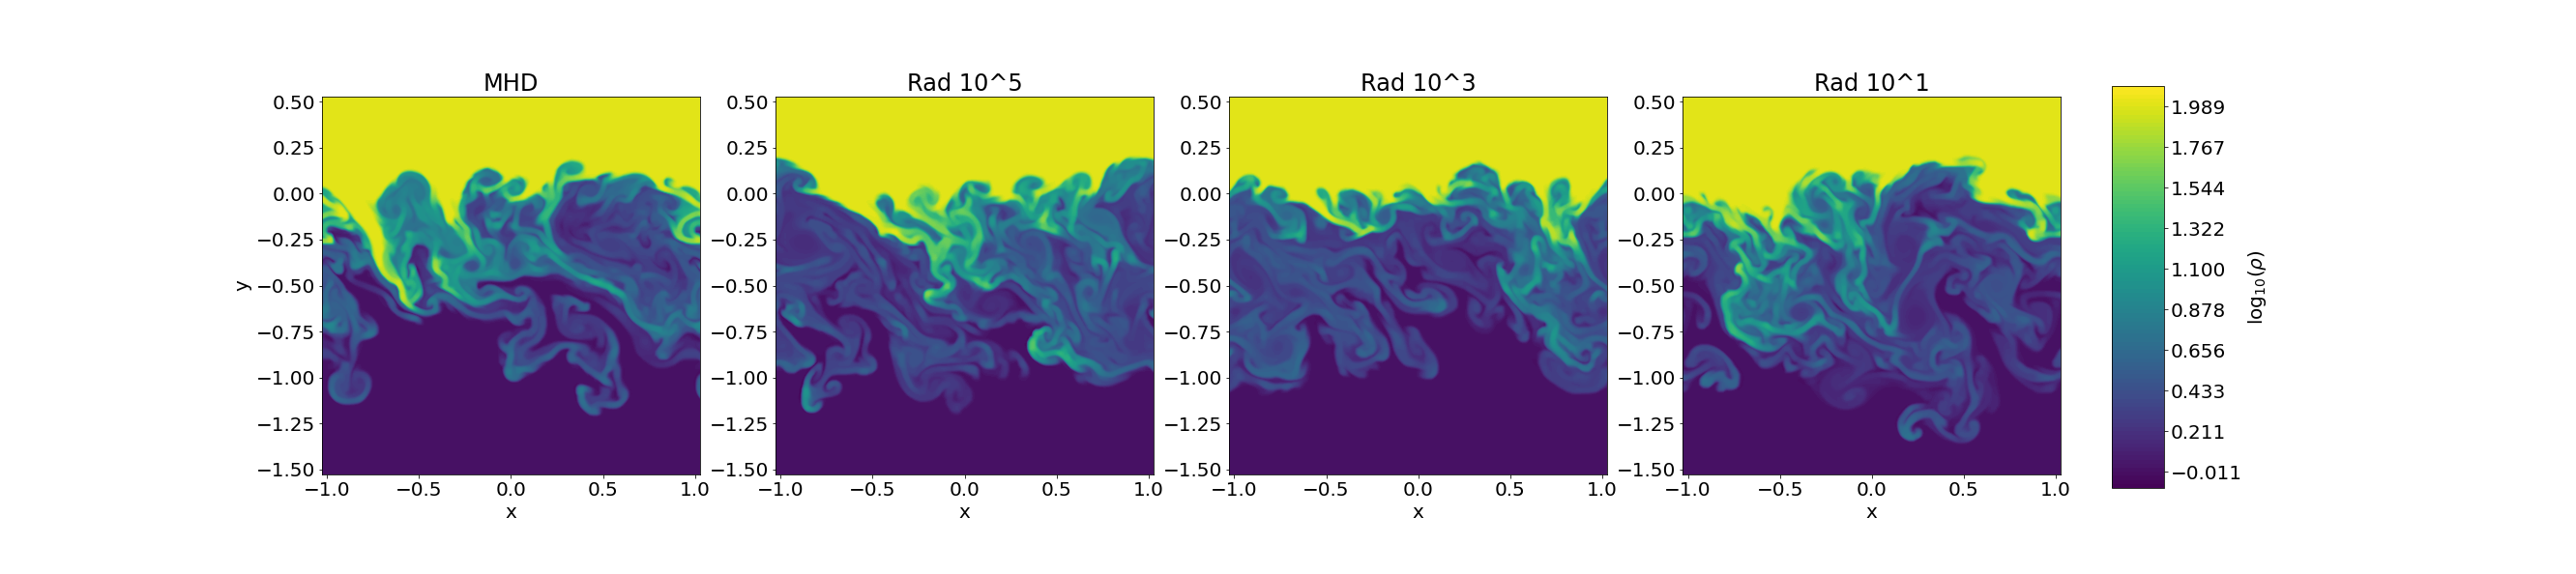
\includegraphics[width=0.99\linewidth,clip=true,trim=58.9cm 0.8cm 8.9cm 0.8cm]{2023Dundee/Figures/denstempevo_rho_t0071.png}
%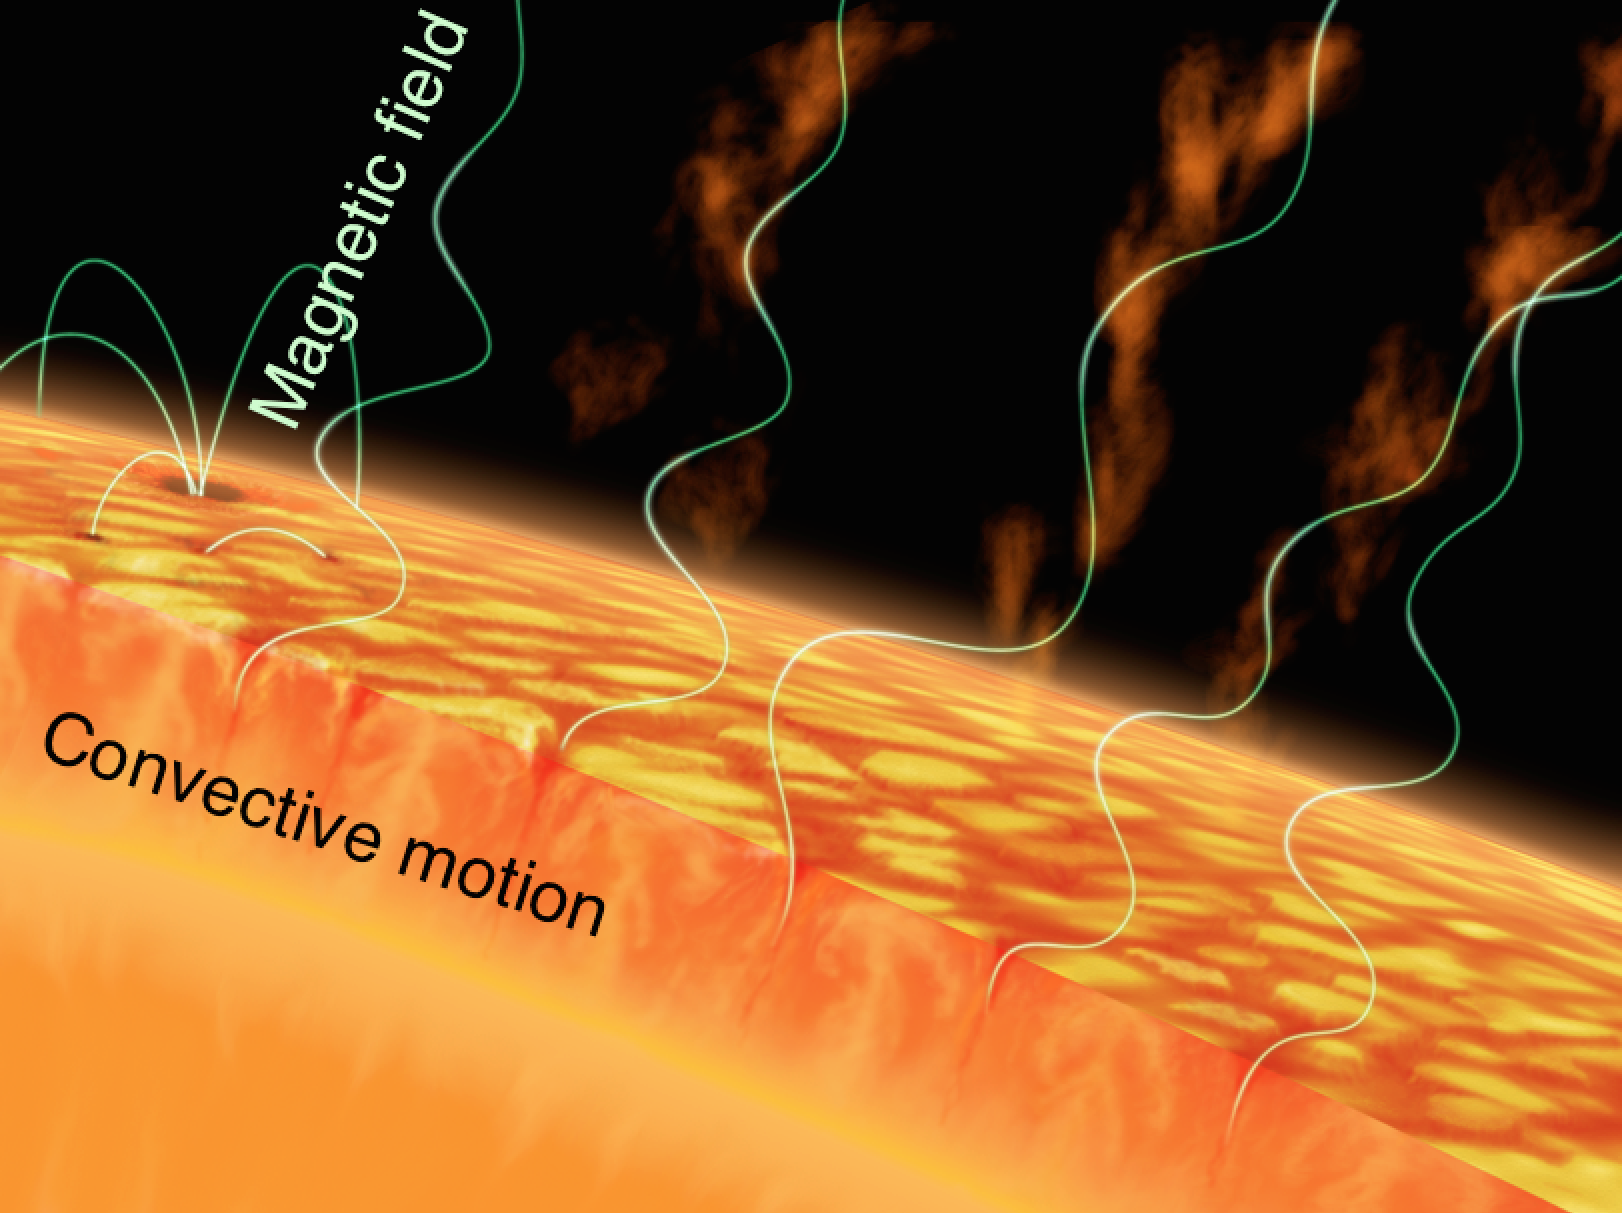
\includegraphics[width=0.95\linewidth]{2023Dundee/Figures/waveheating.png} 
%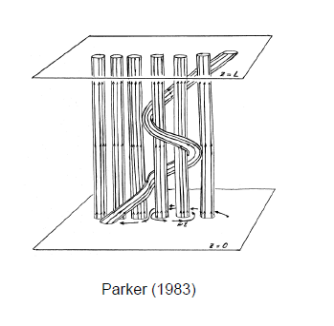
\includegraphics[width=0.95\linewidth]{2023Dundee/Figures/reconnection.png} 
%Conservative equations (e.g., two-fluid with thermal collisions) leads to MHD shock jumps, Snow \& Hillier 2019.
\end{column}
\end{columns}
\end{frame}

\begin{frame}{Conclusions}
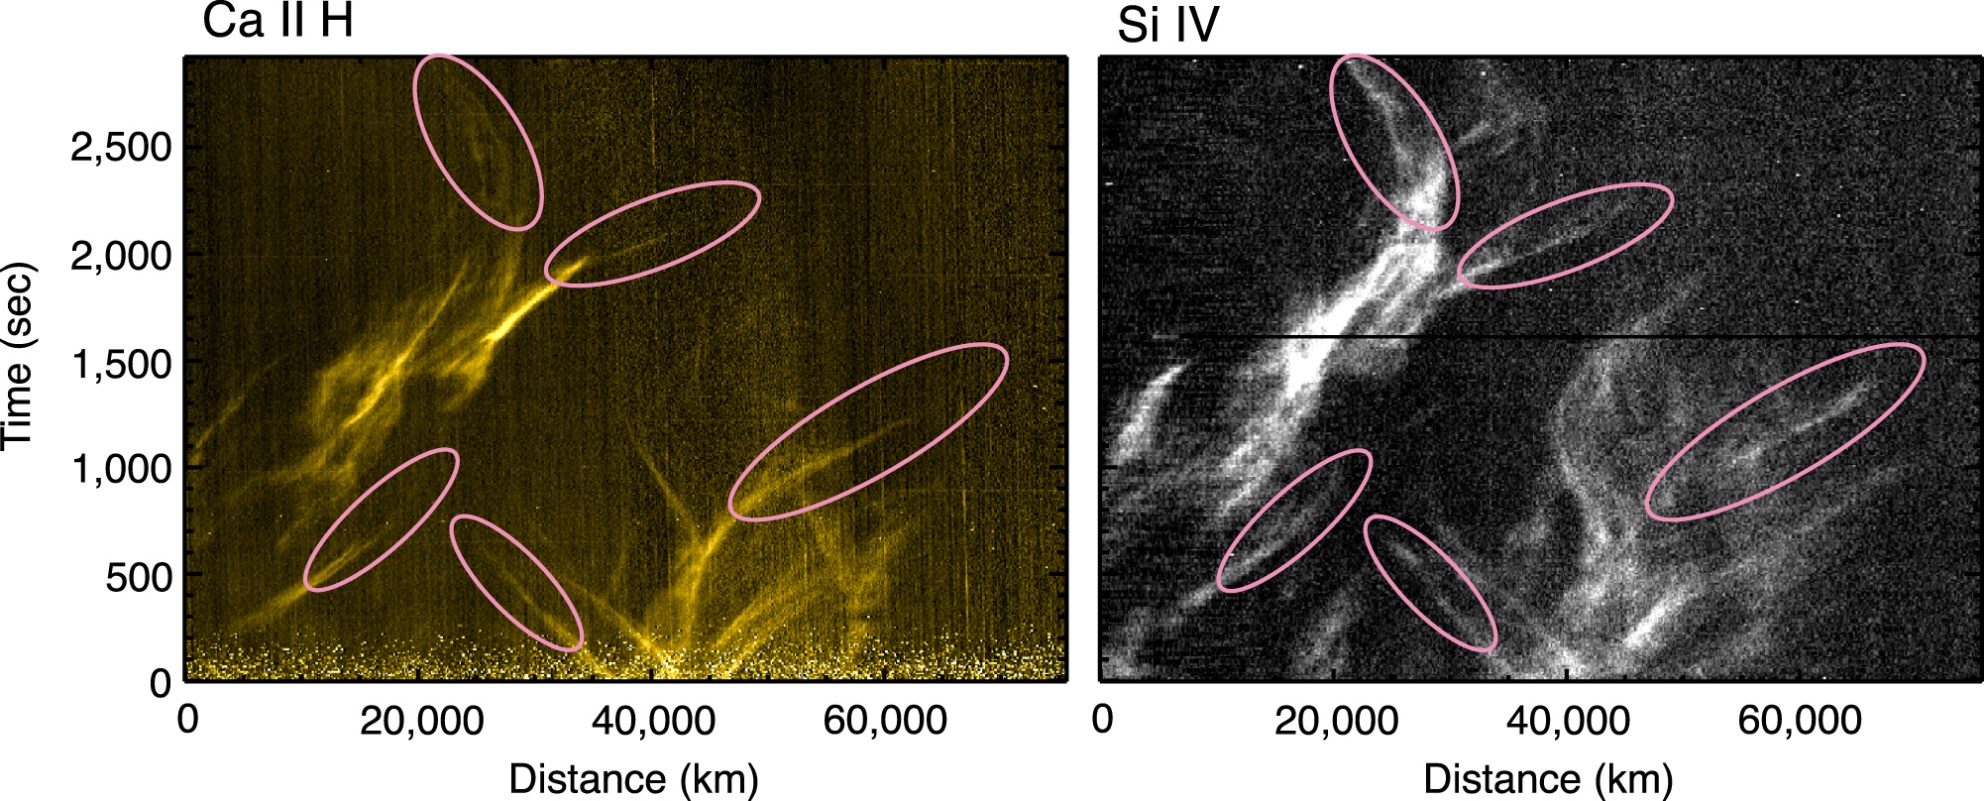
\includegraphics[width=0.95\linewidth]{2023Dundee/Figures/observation.png}
\begin{itemize}
    \item KHI mixing can induce cooling of solar material.
    \item Analytical approximations seem to match the results well for width and loss rate.
    \item Is this observation showing heating or just mixing/cooling?
\end{itemize}
\end{frame}

% \begin{frame}{Maximum theoretical heating/cooling}
% \begin{columns}
% \begin{column}{0.8\textwidth}
% \begin{figure}
%     %\centering
% %    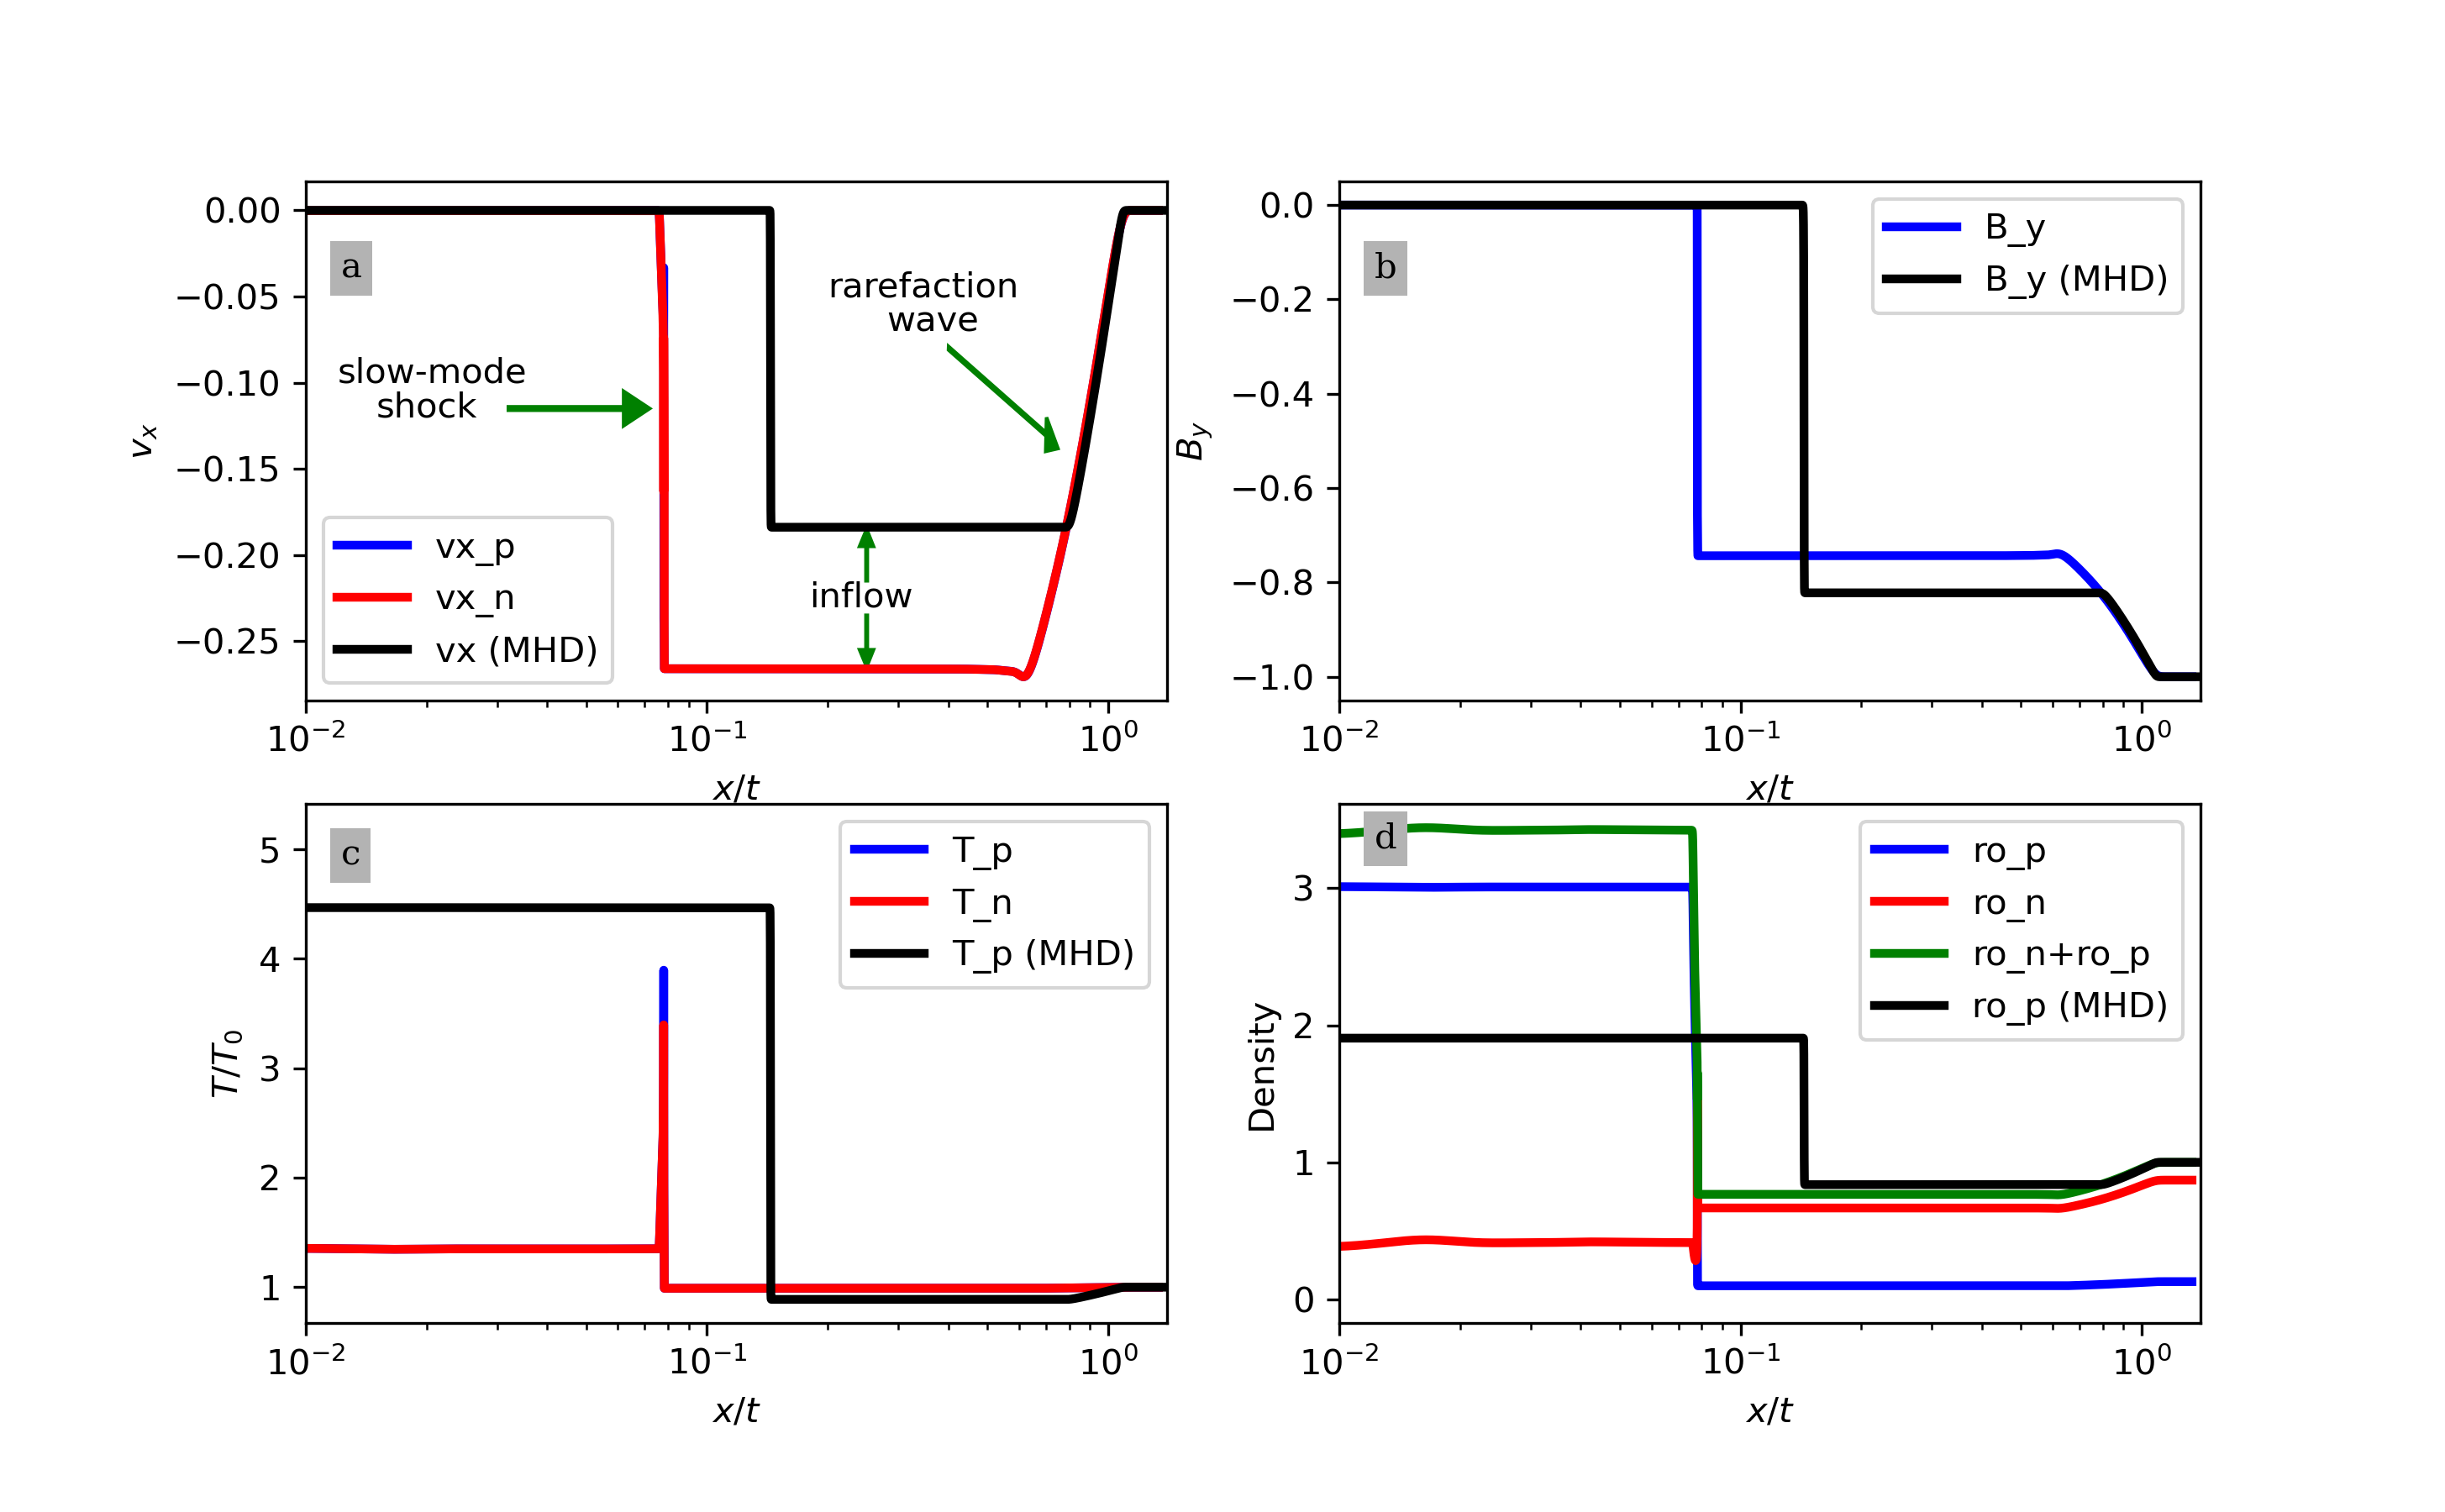
\includegraphics[width=0.95\linewidth,clip=true,trim=0.9cm 0.8cm 0.9cm 0.8cm]{Figures/contextplot.png}
%     %\caption{Upper-chromosphere case showing the $v_x$ velocity (top left), $B_y$ magnetic field (top right), temperature (lower left) and density (lower right). For panel c, the reference temperature $T_0=6220$.}
% %    \label{fig:upperchromocontext}
% \end{figure}
% \end{column}
% \begin{column}{0.2\textwidth}
% %\begin{itemize}
% %    $T_0=6220$, $n_e=7.5\times 10^{16}$, $\xi_n=0.87$
% %\end{itemize}
% \end{column}
% \end{columns}
% \end{frame}

%%%%%%%%%%%%%%%%%%%%%%%%%%%%%%%%%%%%%%%%%%%%%%%%%%%%%%%%%%%%%%%%%%%%%%%%%%%%%%%%%%%%%%%%%%%%%


\end{document}
